\documentclass{WileyMSP-template}
\usepackage[utf8]{inputenc}
\usepackage{textgreek}
\usepackage{bbm}
\usepackage{amsfonts}
\usepackage{amsmath}
\usepackage{longtable}   
\usepackage{booktabs}   
\usepackage{array}  
\usepackage{booktabs}
\usepackage{geometry}
\usepackage{caption}   

\begin{document}


\pagestyle{fancy}
\rhead{\includegraphics[width=2.5cm]{vch-logo.png}}


\title{Deep Learning-Based Emotion Recognition using EEG: A Comprehensive Review}

\maketitle



% Author: Please give full first and last names for authors and include * after the name of all corresponding authors

\author{Shihab Sarar}
\author{Md Niaz Imtiaz*}
\author{Naimul Khan}


% Dedication

\dedication{}

% Affiliations: Please provide adacemic titles (Prof. or Dr.) for all authors where applicable, and include an institutional email address for all corresponding authors
\begin{affiliations}
Shihab Sarar\\
Department of Computer Science and Engineering, Ahsanullah University of Science and Technology, Love Road, Tejgaon Industrial Area, Dhaka-1208, Bangladesh\\
Email Address: shihabsararchamok@gmail.com

Md Niaz Imtiaz\\
Department of Electrical, Computer and Biomedical Engineering, Toronto Metropolitan University, 350 Victoria St, Toronto, ON M5B 2K3, Canada\\
Email Address: niaz.imtiaz@torontomu.ca

Naimul Khan\\
Department of Electrical, Computer and Biomedical Engineering, Toronto Metropolitan University, 350 Victoria St, Toronto, ON M5B 2K3, Canada\\
Email Address: n77khan@torontomu.ca

\end{affiliations}


% Keywords: Please provide a minimum of three and a maximum of seven keywords, separated by commas

\keywords{electroencephalography (EEG); emotion recognition; affective computing; deep learning; cross-subject learning; brain–computer interface (BCI); signal processing}

\textbf{Abstract}

\begin{abstract}
Emotion recognition using EEG is a growing trend in affective computing, with highly fragmented studies regarding datasets, approaches, and evaluation metrics, as well as a high degree of inter-individual variability and a rapidly changing set of deep learning approaches. In this scenario, it is difficult to extract a comprehensive view on the generalizability and practicability of the approaches considered. This work offers a structured review of emotion recognition using EEG, aiming to decrease this level of fragmentation by grouping the existing approaches following signal processing, representation learning, deep learning architectures, and cross-subject learning strategies. The most widely adopted deep learning architectures, graph-based, recurrent, and convolutional neural networks, are considered regarding their set of architectural choices, strengths, and weaknesses, as well as related trade-offs. Other major issues, overfitting, small dataset, and subject dependency, are illustrated and critically considered together with more recent approaches trying to increase the reliability of EEG emotion recognition systems. According to recent studies, the accuracy achieved in subject-specific approaches is higher than 95\%, while for the subject-independent approach, accuracy values vary from 70\% to 90\%, depending on the dataset and the architecture considered.
\end{abstract}


% Text: Please use section headings and subheadings as specified below. For communications, all section headings apart from Experimental Section should be removed
% Please make the first reference to a display item bold: \textbf{Figure 1}
% Do not abbreviate Figure, Equation, etc.; display items are always singular, i.e., Figure 1 and 2.
% Equations are always singular, i.e., Equation 1 and 2, and should be inserted using the {equation} environment, not as graphics
% Please do not use footnotes in the text, additional information can be added to the Reference list.

\section{Introduction}
Emotion recognition is at the heart of models of human behavior, since emotional states directly and profoundly affect human cognition, decision-making, and social interactions. Automatic emotion recognition facilitates the development of intelligent systems capable of adaptively responding to the affect states of users, and this is particularly critical in contemporary human-computer interaction tasks. Emotion recognition in psychology and neuroscience helps in the objective analysis of affective phenomena independently of subjective self-assessments, and in the health sector, it paves the way for numerous tasks, such as the objective evaluation of mood disturbances, patient recovery, and supportive treatment of neurodevelopmental disorders such as autism and affect dysregulation. Emotion recognition in engineering and brain-computer interface studies helps in developing adaptive systems capable of automatically responding to the affective states of users. Emotion recognition using EEG recordings is particularly useful in patient-oriented tasks in the health sector, such as patient recovery and long-term evaluation of patient moods, wherein overt behavioral manifestations of patients could be ambiguous and unavailing. EEG emotion recognition stands distinct, as it directly taps brain signals related to emotion recognition, and this makes the technology valuable in tasks where robustness and physiological validity of the detection tasks are critical.

Electroencephalography (EEG) is a non-invasive neurophysiological sensing technique that records electrical activity generated by neuronal populations with high temporal resolution. Because EEG captures brain dynamics at the millisecond level, it provides fine-grained insight into neural processes underlying emotional responses, which are often transient and rapidly evolving \cite{zheng2015eeg,koelstra2012deap}. EEG-based emotion recognition systems exploit this close coupling between brain activity and affective processing by analyzing neural responses elicited during emotional stimulation to infer underlying emotional states \cite{lin2010eegemotion}. This neurophysiological grounding distinguishes EEG from peripheral or behavioral modalities and motivates its widespread adoption in affective computing research.

EEG further provides important advantages compared to other emotion recognition methods, like facial expressions, speech, or body gestures. Behavioral cues are susceptible to intentional control, social camouflage, and context effects and are thus not very reliable in a sensitive context.  Conversely, EEG oscillations are symptomatic of inner neural activities that are hard to manipulate intentionally and supply objective estimations of affective states \cite{craik2019deep}. Although increasingly explored, at least for the future of emotion-sensitive BCIs, multimodal approaches combining EEG with other physiological or behavioral signals are not required, and EEG alone can be a robust and informative modality owing to its direct sensitivity to emotional brain dynamics and the compatibility with BCI systems.

Despite having all these benefits, there are a few challenges to recognizing emotions using EEG. The quality of an EEG signal is highly dependent on factors like electrode positioning, skin conductance, movement artifacts, and inter-session inconsistency. Variability in experimental procedures, emotional stimuli used, labeling approaches, and preprocessing techniques adds to inconsistencies \cite{alotaiby2017review}. These create difficulties in comparing methodology-based approaches systematically, especially when assessing performance on diverse databases such as DEAP, SEED, and DREAMER \cite{koelstra2012deap,katsigiannis2017dreamer}. Additionally, large variations between subjects lead to large distribution changes in the features of an EEG signal, thereby negatively affecting subject-independent generalization.

Recent breakthroughs in deep learning have led to significant improvements in EEG-based affect recognition models that are capable of learning informative features directly from raw or lightly preprocessed signals \cite{craik2019deep}. Convolutional Neural Networks (CNNs) capture channel-level relations in EEG signals \cite{li2018cnn}, Recurrent Neural Networks (RNNs) model temporal dependencies in brain activity dynamics \cite{yang2018rnn}, and Graph Neural Networks (GNNs) represent task-relevant functional connectivity between brain regions \cite{wang2022gcn}. Despite their strong ability in achieving a high level of accurate classification for subject-dependent tasks, they have been observed to have poor generalization capability for cross-subject and cross-corpus \cite{zhang2021cross}.

There has been an increased need to carry out a review of up-to-date research work in the area of emotion recognition using EEG. There are many reviews that were mainly concentrating on architectural originality or evaluation tasks on a single dataset, with less concern for cross-subject and cross-dataset generalization \cite{alotaiby2017review,craik2019deep}. Additionally, a lack of standardized preprocessing pipelines and inconsistencies in evaluation methodologies make it hard to make a valid inference \cite{peerjreview2023} on the research. There is no consensus or agreement on the best way for model design, evaluation, and implementation of effective EEG-based emotion recognition \cite{springerreview2024}.

Limitations of some of the above-mentioned works have only focused on one aspect of deep learning for EEG-based emotion recognition. In order to overcome these limitations, this paper provides a systematic and detailed review of deep learning methods for EEG-based emotion recognition. The key contributions of this review are summarized as

\begin{enumerate}
    \item A well-organized establishment of fundamental research issues pertaining to processing and feature extraction of EEG signals, as well as deep learning-based modeling of emotion.
    \item Comparative synthesis of CNN, RNN, and GNN-based approaches within subject-specific and subject-independent frameworks.
    \item Discussion of generalization, robustness, and efficiency tradeoffs in paradigms of deep learning analytically.
    \item Critical analysis of existing work on transfer learning and domain adaptation methods for dealing with intersubject and cross-dataset variation.
\end{enumerate}

This review integrates scattered research on EEG emotion recognition into a cohesive view. It provides an overview of the essential challenges of EEG signal processing, feature extraction, and deep learning for modeling emotions and comparisons of popular neural architectures like convolutional networks, recurrent networks, and graph networks for subject-specific and subject-independent tasks. This review provides an insight into the essential trade-offs of generalization capability, robustness, and complexity that limit the application of the current solutions. Apart from this, the potential of transfer learning and domain adaptation in handling intersubject and cross-domain variability has been discussed with both limitations and opportunities. There are several other topics that will be discussed in the review to introduce an overview of the state of the art while identifying the essential research paths for improving robust and scalable solutions for EEG emotion recognition.

\section{Theoretical and Methodological Foundations}
The theoretical background defines EEG-based emotion recognition as a framework that links measurable neurophysiological activity to computational representations of affect. It models emotional state as a structured pattern distributed across time, frequency bands, and scalp locations, and it treats learning as the problem of extracting robust features or representations from noisy, non-stationary brain signals \cite{wang2024researchprogress}. It also establishes the use of emotion label names via two-way paradigms: the discrete classification paradigm, where EEG segments are classified into distinct affective states, and the continuous modeling paradigm, where predictions of valence and arousal ratings are performed \cite{ma2024peerjreview}. These standpoints shape design decisions, evaluation schemes, and generalizations over subjects and sessions \cite{li2022transferreview}.

\subsection{Emotion Recognition}
Emotion recognition is a principal goal of affective computing in pursuing the aim of enabling computational systems that can efficaciously and adaptively respond to the emotional states of humans. Notwithstanding the increasing penetration of human-computer interaction into more and more areas of everyday life, the overall lack of awareness of user emotional states in human-computer interfaces hampers the overall efficiency of such interfaces in applications that demand user-level personalization, empathy, and commitment to user well-being, thereby pursuing the need to endow computers with the potential to identify user affective states through some form of user cues or physiological signals.

Conventional emotion recognition methods exploit behavioral features, such as facial expression, speech pattern, body language, and text messages. Though these features express more palatable aspects of human emotion, they are still amenable to control and masking in a controlled manner. In this context, combining different sources of variation with physiological measures, which are less controllable at a voluntary level, constitutes a more objective solution. Among various physiological measures, EEG represents a prominent choice because of its direct sensitivity to neural mechanisms related to processing emotions and its high resolution, enabling the monitoring of rapid dynamics of emotions \cite{ma2024peerjreview,hamzah2024heliyon}.

EEG-based emotion recognition systems model tasks that relate to EEG-stimuli pairs distributed with certain emotion categories. The changes in the emotional state cause changes in EEG rhythms and spatial activity, as well as changes that could be used to extract new information on state transitions between different emotions. According to a set of recent surveys on EEG-based emotion recognition models, the traditional pipeline of EEG emotion recognition systems includes data processing, noise removal, eigenvector transformation, and machine learning inference, with a current emphasis on end-to-end models. Traditionally, models are based on some hand-engineered features from temporal, frequency, or time-frequency worlds, whereas current models are increasingly based on deep learning models that extract hierarchical features from EEG data.

Deep learning models have characterized the emotion recognition study area because of their ability to learn complex, non-linear correlations in multichannel EEG data. Convolutional neural networks have been extensively employed to leverage the spatial information among EEG electrodes, mostly applied when processing EEG maps or image-like representations of EEG signals. Recurrent and Gated Recurrent Neural Networks have been used to model time information, and their primary purpose is to capture time-dependent information of emotion relevant to the research area. Most of the recent studies incorporated graph neural networks and leveraged the connectivity between EEG channels, which gives neurobiologically valid models for emotion recognition \cite{li2022transferreview,ma2024peerjreview}.

Despite improvements in algorithm methodology, emotion recognition accuracy is known to remain highly vulnerable to specific experimental conditions. In subject-dependent approaches, the absence of significant variability leads to excellent accuracy, while subject-independent and cross-dataset approaches remain significant challenges \cite{li2022transferreview,hamzah2024heliyon}. Variability across people and recording devices, as well as divergence across protocols for invoking emotions, causes substantial distribution divergence, thereby negatively impacting overall generalization. Thus, there is a growing trend within recent studies on applying transfer learning, domain adaptation techniques, and alignment techniques for enhanced subject and recording device independence \cite{li2022transferreview,hamzah2024heliyon}.

Emotion recognition is viewed in the literature not only as a classification problem but also as a much more complex inference problem, which is affected by neurophysiological variations, experimental conditions, and generalization. Continued progress in EEG-based emotion recognition, therefore, depends on jointly advancing acquisition protocols, representation learning, and evaluation methodologies to support reliable deployment in real-world affective systems.

\subsection{Neurophysiological Foundations of Emotional States}
Neurophysiological accounts of emotion in EEG-ER interpret emotional episodes as changes in distributed brain activity that manifest as time-varying and band-limited oscillatory patterns across channels. EEG acquisition during affective stimulation, therefore, produces signals with \emph{spatial structure across electrode locations, temporal structure due to stimulus duration and sliding-window segmentation, and frequency structure because analysis commonly separates δ, θ, α, β, and γ rhythms, each of which exhibits different responsiveness under affective conditions} \cite{wang2024researchprogress}.

Within this framing, EEG-ER pipelines either follow a staged procedure (denoising → feature extraction → classifier learning) or adopt end-to-end feature learning, and they rely on assumptions about label availability and the degree to which training and test data approximate i.i.d. conditions \cite{li2022transferreview}. When these assumptions fail—especially under cross-subject, cross-session, or cross-database settings—emotion-related neural patterns appear heterogeneous, motivating modeling strategies that explicitly target domain gaps and subject bias \cite{li2022transferreview}.
EEG-ER surveys formalize feature construction as multi-domain representation learning. Temporal features describe transitive or long-term variations of events, while spectral features are the result of band-pass filtering, Fourier transforms, and other transforms like it. Spatial features describe inter-channel relationships that correspond to the spatial organization of the cortical structure of the human brain and its variability \cite{wang2024researchprogress}. This multi-domain stance links directly to contemporary architectures (CNN/RNN/GNN/Transformer variants) that operationalize spatial-temporal-spectral fusion and to transfer-learning approaches that seek domain-invariant representations under strong inter-individual variability \cite{geng2025dlreview}.

Benchmark datasets encode these neurophysiological assumptions by pairing affective stimuli (e.g., videos/music) with EEG recordings and either discrete labels or continuous ratings, thereby defining the target emotional state space and the evaluation protocol \cite{li2022transferreview}.

\subsubsection{Discrete Emotion Representation Models}
Discrete EEG-ER models treat emotion as membership in a finite set (e.g., positive/neutral/negative; basic categories), and they implement classification as a mapping from multi-channel EEG representations to class labels. The literature consistently organizes discrete modeling around (a) feature engineering or learned representations across temporal–spectral–spatial domains and (b) classifier families ranging from SVM/KNN to deep neural architectures \cite{wang2024researchprogress}.

A core empirical regularity in discrete EEG-ER is that frequency-domain features—including PSD and differential entropy—serve as widely used affective descriptors, commonly computed per band and per channel before classification \cite{ma2024peerjreview}. Discrete pipelines, therefore, often couple bandwise features with spatial modeling to reflect the channel topology, using methods such as CSP/HDCA for spatial structure or deep models that internalize spatial priors \cite{ma2024peerjreview}. 

Additionally, deep learning reviews break down the most popular discrete EEG-ER models into single models: CNN/RNN/GNN models, attention models, combination models, and domain transfer models or models that perform DG/DPre \cite{geng2025dlreview}. According to the categories of the above review, the most popular discrete models are the following: DEAP-discrete models of CNN models \cite{tripathi2017deapcnn}, hierarchical CNN models of DEAP data that use natural spectral features like differential entropy maps \cite{li2018hcnn}. RNN/GRU/LSTM variants implement the concept of temporal dependency, such as attention-driven LSTM classifiers and spatiotemporal recurrent designs \cite{kim2020lstmatt}. Parallel convolutional–recurrent designs explicitly fuse spatial filtering with temporal recurrence in multi-channel EEG \cite{yang2018pcrnn}. GNN-based discrete EEG-ER models represent electrodes as nodes and learn adjacency structures to encode functional coupling patterns \cite{zhong2020rgnn}.

Discrete state modeling also depends on the experimental regime. Surveys separate subject-dependent and subject-independent protocols because cross-subject generalization remains harder and motivates architectural choices (e.g., graph attention, domain adversarial training) and evaluation practices \cite{ma2024peerjreview}. In this context, domain adaptation methods and adversarial learning explicitly address subject bias by aligning feature distributions across individuals \cite{geng2025dlreview}. 

The transfer-learning approaches for EEG-ER problems further solidify discrete EEG-ER as a problem of learning over gaps within domains owing to differences within the subject, session, or database. Domain transfer for knowledge can be classified along the lines of instance transfer, feature transfer, parameter transfer, and relation transfer, each dealing with the discrete classification problem through minimizing the discrepancy over domains \cite{li2022transferreview}. Methods, for instance, weight assignment as in TrAdaBoost, seek to weight the source instances to align with the target domain \cite{li2022transferreview}. Others apply feature transformation or learn subspaces to reduce distribution discrepancy and include deep learning approaches that learn transfer representations \cite{li2022transferreview}. The methods for parameter transfer encompass model fine-tuning and transductive parameter transfer, making effective use of model portability across domains \cite{li2022transferreview}. 

Discrete models also incorporate label sets that are specific to the data sets. Discrete sets of categories such as anger, fear, sadness, and happiness, among others, are commonly found in public databases, and they can also help in a comparative study \cite{li2022transferreview}.

\subsubsection{Continuous Dimensional Emotion Representation Models}
Continuous EEG-ER models treat emotion as a point in a low-dimensional affective space (most commonly valence–arousal, sometimes extended with dominance/liking/familiarity), and they implement learning as regression, ordinal prediction, or discretization of continuous ratings into quadrants/bins. Reviews emphasize that datasets explicitly differ in whether they provide continuous ratings or discrete labels, and they organize benchmark corpora accordingly \cite{wang2024researchprogress}.

From a neurophysiological perspective, continuous modeling aligns with the idea that EEG dynamics vary smoothly over time and that affective response strength differs across frequency bands and windows; thus, temporal segmentation and band decomposition are foundational operations before continuous inference \cite{wang2024researchprogress}. Continuous systems typically compute bandwise features (PSD/DE/entropy) or learn representations end-to-end, and they map these representations to dimensional ratings using neural regressors or hybrid architectures \cite{li2022transferreview}.

Continuous emotion modeling also inherits the central challenge of domain gaps. Transfer-learning surveys define cross-session transfer as addressing acquisition-time variability within the same subject and define cross-subject transfer as addressing individual differences; both scenarios directly affect dimensional prediction because rating scales must remain comparable while EEG distributions shift \cite{li2022transferreview}. Cross-database transfer further compounds these difficulties due to differences in devices, experimental conditions, and label distributions, making it the most challenging scenario for stable continuous inference \cite{li2022transferreview}.

\begin{figure}
    \centering
    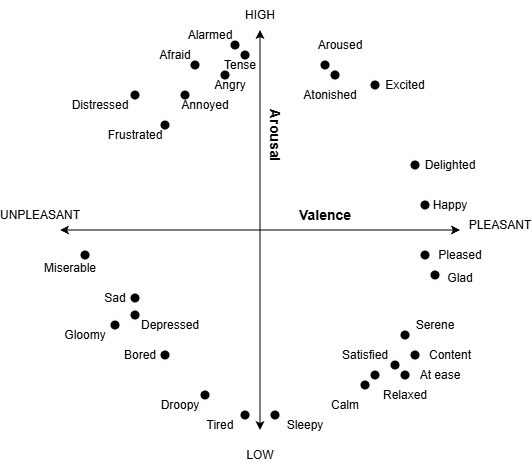
\includegraphics[width=0.5\linewidth]{pictures/Valence.png}
    \caption{Valence-Arousal 2D Affective Model}
    \label{fig:valence}
\end{figure}

In practice, continuous EEG-ER systems often discretize ratings into two-class (high/low) or four-quadrant valence–arousal tasks to enable comparability with classification pipelines while preserving the underlying dimensional semantics \cite{wang2024researchprogress}. Surveyed results illustrate that some methods explicitly evaluate both binary dimensional splits and quadrant partitions on datasets such as DEAP and DREAMER, reflecting a continuum between regression-style modeling and discretized dimensional classification \cite{wang2024researchprogress}.

Deep learning reviews indicate that architectures used for continuous affect frequently mirror those used in discrete settings—CNNs for local spatiotemporal patterns, RNNs/GRUs for sequential structure, and attention mechanisms for adaptive weighting—while evaluation emphasizes stability and generalization across subjects, which remains more challenging but more deployment-relevant \cite{geng2025dlreview}. Another factor, according to survey studies, is that EEG signal processing and feature extraction are still very important, given the presence of noise in EEG signals, which require signal denoising and robust representation learning for predictive processing \cite{li2022transferreview}.

Transfer learning becomes especially relevant in continuous affect because it reduces target-domain labeling demand by transferring learned structure from related subjects/sessions/databases, but it also introduces risks of negative transfer when domain gaps are large \cite{li2022transferreview}. Consequently, feature-based deep transfer learning (e.g., discrepancy minimization and adversarial alignment) emerges as a dominant direction for improving dimensional generalization \cite{li2022transferreview}.

\subsection{Emotion Induction and Stimulus Design}
Emotion induction and stimulus design determine how affective responses are reliably evoked and temporally aligned with EEG recordings. Prior methodological surveys describe emotion induction as a prerequisite for meaningful EEG labeling, because weak or inconsistent stimuli directly degrade the validity of learned affective representations \cite{alarcao2019eegsurvey}. Paradigms involving images, music, or video clips remain popular paradigms because they ensure accurate onset-offset timing, which also ensures easy repeated measurement for every participant, helping in easy segmentation and extraction of features \cite{roy2019dleegreview}. These paradigms also involve post-trial self-evaluation tasks for mapping brain responses with subjective experience in order to reinforce the accuracy of labeling at the trial level \cite{jafari2023dlreview}.

\begin{figure}[htb]
    \centering
    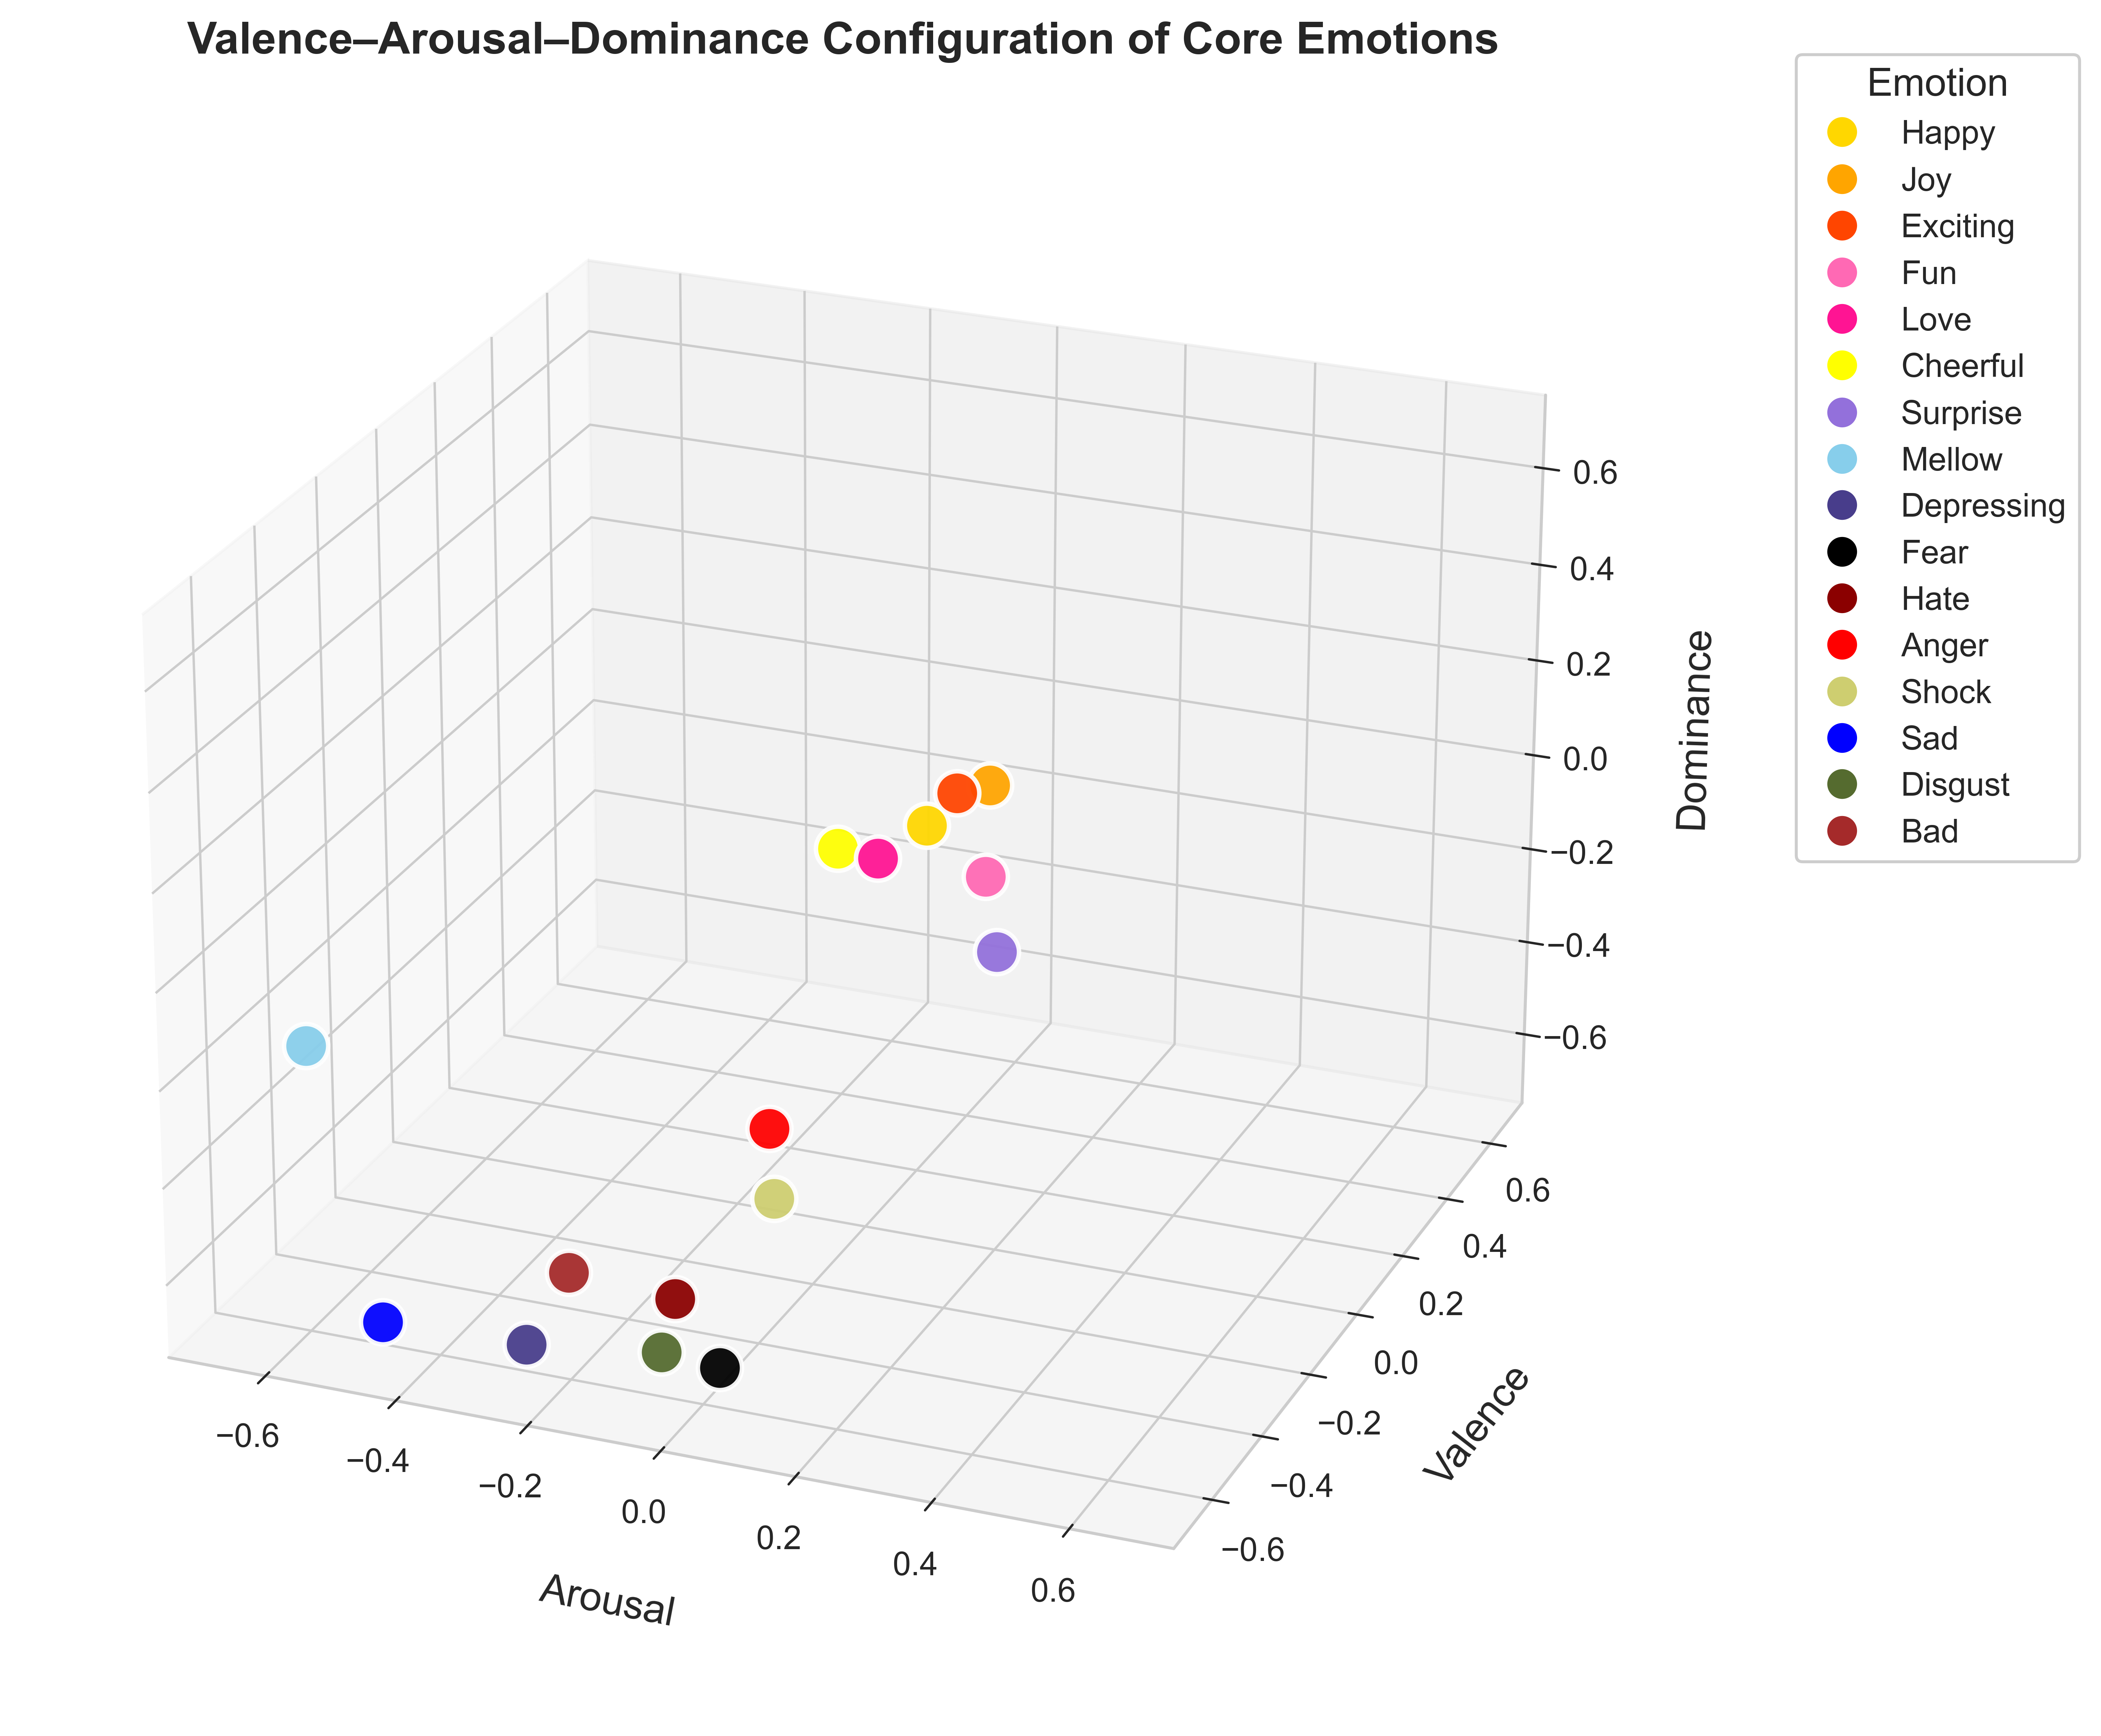
\includegraphics[width=0.6\linewidth]{pictures/3D_emotion.png}
    \caption{Stimulus}
    \label{fig:stimulus}
\end{figure}

Interactive and task-driven stimuli are growing in usage as alternative paradigms because they promote enduring and contextually rooted emotion processes that passive stimuli may fail to support. However, the literature underscores that such paradigms significantly amplify inter-subject variability as well as the overall complexity of the experiments \cite{lu2021bcisurvey}. Memory recall methods based on the subject's personal memory rely on personal emotion triggers but fall prey to personal cognitive and emotion variables; therefore, their cross-subject universality is limited \cite{wan2021tleeegsurvey}. In summary, modern studies on emotion processing with the EEG directly address the issue of stimuli as a trade-off between standardization, engagement, and universality \cite{wu2020tleeegbci}.

In terms of stimulus modality, the scope of induction practice also extends towards the integration of multimodal signals (such as peripheral physiology and facial expressions) in order to check if the target affective state can be expressed uniformly across the trials, which favors temporal synchronization between subjective states and physiology targets \cite{rayatdoost2020expressionguided}. Cross-corpus evaluation also favors stimulus calibration, as differences in the content of elicitation can contribute towards the shift problem in EEG representations of affect \cite{rayatdoost2018crosscorpus}. In addition, modern learning strategies (e.g., contrastive and self-supervised representation learning) encourage elicitation designs that produce diverse yet label-consistent trials, since representation objectives benefit from repeated exposure to comparable affective episodes under varying contexts \cite{shen2022contrastive}. These developments sit naturally within the continuous affect tradition, where valence–arousal modeling formalizes emotion as graded dynamics rather than rigid categories. Finally, the broader affective-computing literature shows that robust elicitation and labeling practices generalize across biosignals (e.g., ECG as well as EEG), reinforcing the view that stimulus design functions as a system-level determinant of downstream generalization \cite{sarkar2020selfsupervised}.

\subsection{Progress in Data Acquisition Technologies}
The development of EEG acquisition equipment is the basis for the development of EEG-based emotion recognition research. The early study of affective brain activity mainly used research-grade EEG systems characterized by high-density electrode arrays, gel-based sensors, and shielded laboratory settings; these provide a high signal-to-noise ratio and also very accurate spatial resolution, which is a requirement for finding the cortical dynamics of emotions reliably. However, their high cost, time-consuming setup, and participant discomfort make it difficult to scale and be practical for real-world scenarios of emotion recognition. As emotion recognition research gradually shifted from highly controlled laboratory studies toward applied and real-life contexts, the limitations of traditional EEG hardware became obvious.

EEG acquisition hardware also plays a significant role in the data’s quality, the model's generalization ability, and the system’s feasibility for use in the real world for emotion recognition systems. Hardware factors such as EEG electrodes, channels, stability of signals, and resistance to movements also affect the reliability of the acquired feature for emotions. Emotion recognition systems trained to recognize data from research acquisition systems find it difficult to generalize and recognize signals originating from consumer acquisition systems or wireless acquisition systems for data collection. Thus, acquisition system selection is not just a design choice but now a deliberate factor in model performance between subjects, data set transferability, and feasibility for use in the real world for human-computer interaction, wearable healthcare applications, or affective computing systems.

\begin{figure}
    \centering
    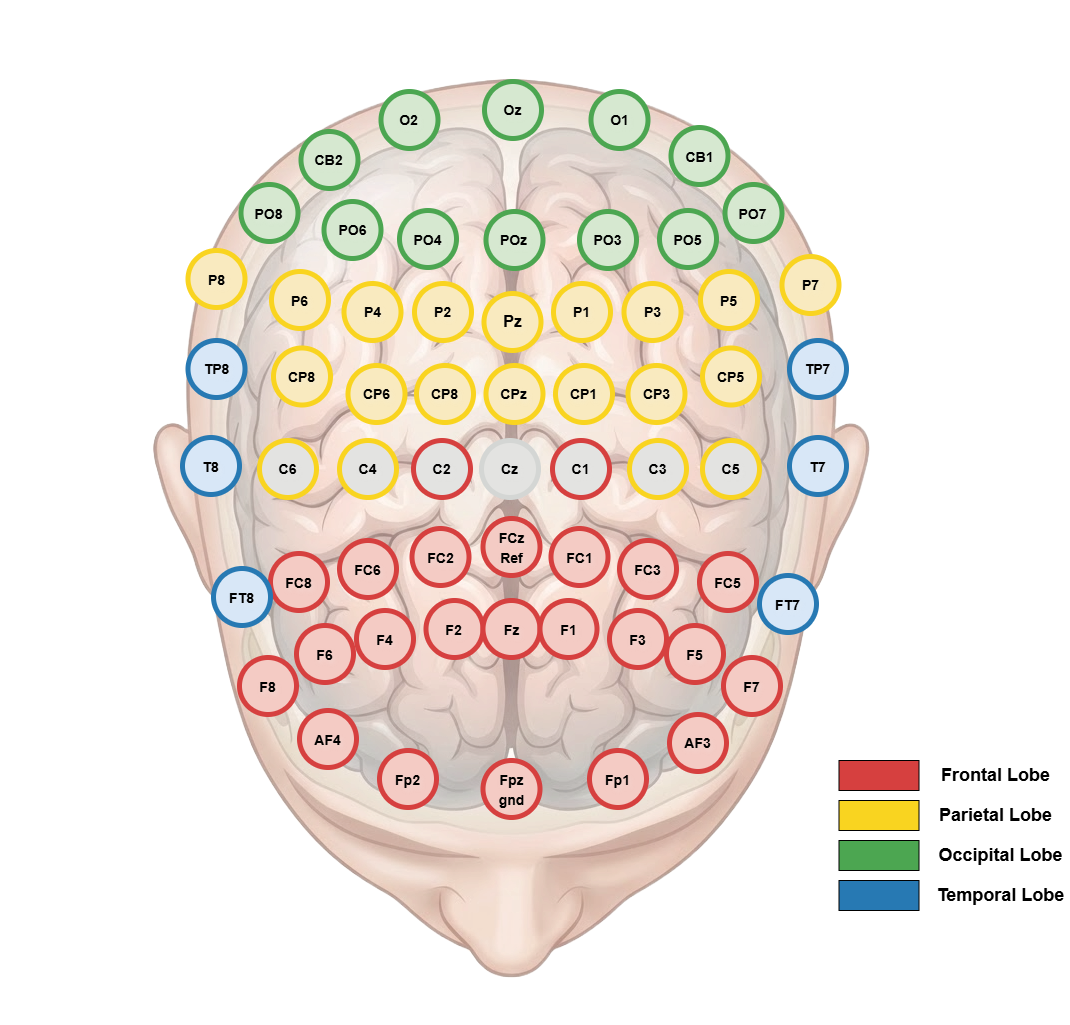
\includegraphics[width=0.6\linewidth]{pictures/Human_Brain_EEG.png}
    \caption{EEG Electrodes}
    \label{fig:electrodes}
\end{figure}

Hairston et al., \cite{hairston2014usability}, in their discussion on various usability problems in conventional EEG methods used for affective computing, focus on the problems caused by the use of 'gel electrodes' and the 'lack of mobility' of the user, though these methods are sure to produce a high degree of data clarity. Debener et al. \cite{debener2012mobile} present the use of mobile EEG equipment that allows for the performance of tests while performing naturalistic procedures, showing the viability of the analysis of related EEG-based emotions. Nevertheless, the raised sensitivity to motion and environmental noise is considerable. On the other hand, wearable equipment with EEG systems, including wireless transfer technology for the continuous monitoring of patients, has also been suggested by Casson et al. in \cite{casson2010wearable}. Although the use of such equipment promotes mobility along with compliance in patients, the number of channels in wearable equipment tends to be reduced, which might influence the emotion classification accuracy. Grozea et al., in their article \cite{grozea2011bristle}, develop a type of dry electrode based on a bristle to reduce gel preparation without adversely affecting signal quality. This reduces not only the discomfort in gel preparation but also improves overall signal quality through minimal head movements or extended period recording. 
Huang et al. \cite{huang2015comb} proposed comb-shaped active dry electrodes for improved scalp coupling. As more robust design solutions are developed for dry electrode upgradation, the increased complexity and cost of such manufacturing processes hinder their acceptability. Zhao et al. \cite{zhao2019calibration} explore short-calibration EEG systems with reduced channel configurations in emotion recognition, demonstrating that affective cues can be preserved even through an optimized preprocessing approach. Nevertheless, the reduced spatial resolution limits the analysis of fine-grained patterns of emotions. To compare the performance of real-time EEG signal processing carried out with consumer-grade devices, the paper by Mullen et al. \cite{mullen2015realtime} shows the impact of domain shifts due to differences in equipment and the need for effective learning schemes. OpenBCI studies \cite{openbci2013} have shown that low-cost and open-sourced EEG data acquisition platforms are well-suited for large-scale experimentation efforts. Nevertheless, low fidelity and improper placement of electrodes are still some key barriers to achieving the goal of accurate emotional recognition.

The advancement of EEG data acquisition equipment can be seen as a good example of a trade-off balancing the quality of the data with the real-world applicability of the equipment itself. Investigational equipment maintains the ability to acquire the best quality data in terms of foundational research, but wearable-style equipment can greatly help in the scalable use of emotion recognition in real-world applications. Although the advancement in terms of the use of dry sensors, wireless data transfer, and in-data-conditioning can help in the reduction of the barriers associated with the use of the equipment itself, the process still needs the acknowledgment of the importance of the role of EEG data acquisition equipment in the emotion recognition system itself, balancing all the strategies in the process in order to achieve the most successful result in real-world use cases.

\begin{table}[t]
\centering
\caption{Association between major cerebral regions and commonly observed EEG frequency bands.}
\label{tab:brain_eeg_mapping}
\begin{tabular}{ll}
\hline
\textbf{Brain region} & \textbf{Dominant EEG frequency bands} \\
\hline
Frontal lobe & Theta (4-7 Hz), Beta (13-30 Hz), Gamma ($>$30 Hz) \\
Temporal lobe & Theta (4-7 Hz), Alpha (8-13 Hz), Gamma ($>$30 Hz) \\
Parietal lobe & Alpha (8-13 Hz), Beta (13-30 Hz) \\
Occipital lobe & Alpha (8-13 Hz; dominant), Beta (13-30 Hz) \\
Central (sensorimotor cortex) & Mu rhythm (8-13 Hz), Beta (13-30 Hz) \\
Limbic-related regions (indirect EEG influence) & Theta (4-7 Hz), Gamma ($>$30 Hz) \\
\hline
\end{tabular}
\end{table}

\begin{figure}
    \centering
    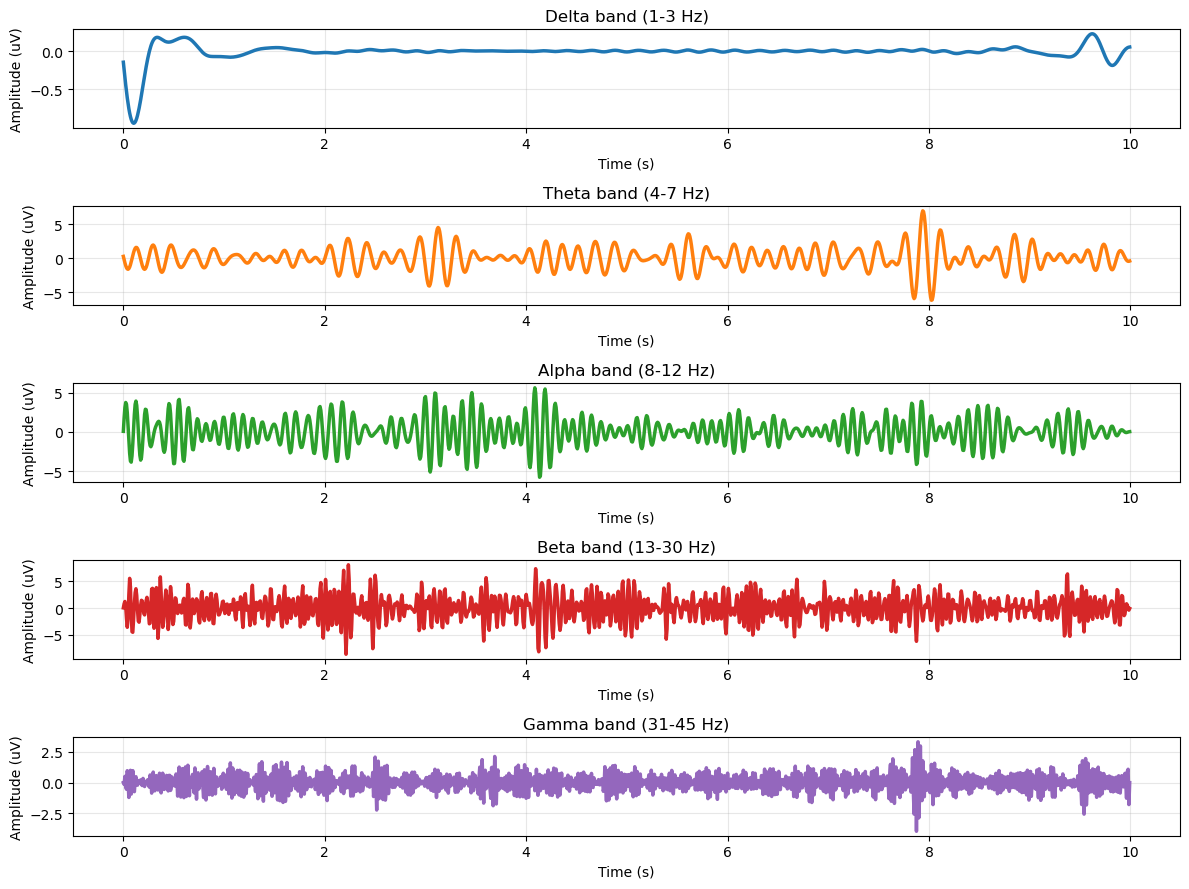
\includegraphics[width=0.7\linewidth]{pictures/Bands.png}
    \caption{Bands}
    \label{fig:bands}
\end{figure}

\subsection{Multimodal Emotion Modeling}
Multimodal emotion modeling appears as an alternative solution for the deficiencies in unimodal systems due to their susceptibility to noise and contextual variations in interpreting the emotional state \cite{soleymani2017survey}. Nevertheless, human emotional responses arise through various modalities such as facial, vocal, and physical communication, which convey valuable personal affective-related communication in addition to individual sources \cite{baltrusaitis2019multimodal}. Thus, through the process of integrating multiple sources of communication, the overall view and understanding of personal emotional state and responses remain contextual \cite{baltrusaitis2019multimodal}.

Emotion analysis in a multimodal environment merges behavioral responses such as facial, speech, text, and gesture signals with physiological signals including EEG, ECG, EMG, GSR, and respiration \cite{d2018physioaffect}. External behavioral responses mainly focus on actual emotional responses. EEG focuses on internal brain aspects of affective responses that are inaccessible for conscious experience \cite{ma2024peerjreview}. EEG helps focus these responses in a temporal manner, relating them to actual emotional responses, at the neural level. They play a significant role in responding to subtle affective responses that might not be captured by other signals. The blend of EEG with the above signals helps make these responses more universally applicable.

It is reported in the literature \cite{baltrusaitis2018multimodal} that multimodal fusion paradigms, each of which corresponds to a different level of integration of cross-modal information, such as \emph{early, intermediate, and late}.

Chen et al. \cite{chen2018featurefusion} investigate early fusion by combining features from EEG, facial, and speech modalities before classification; improved results are shown when feature normalization and synchronization are appropriately applied. However, early fusion is generally plagued by the growth of dimensionality as well as increased sensitivity to misalignment across modalities, complicating training and potentially degrading performance when features are high-dimensional or poorly synchronized. Kessous et al. \cite{kessous2017multimodal} have also applied feature-level fusion in multimodal emotion tasks, where the results show that appropriate preprocessing enhances recognition but such approaches remain challenged by noise and feature heterogeneity across channels.

Proposals for intermediate fusion methods have been developed by Shin et al., \cite{shin2017complex} in which asynchronous modality combination makes use of temporal modeling and sequence alignment. Although this method improves on handling temporal discrepancies between modalities such as EEG and other modalities, it imposes additional complexity in terms of computation. Furthermore, in a different approach based on deep contextual modeling of asynchronous modalities, Liu et al. \cite{liu2024multimodal} utilize intermediate fusion; however, this has limitations in terms of high requirements for training data and in handling long-range dependencies.

Wang et al. \cite{wang2018decisionfusion} delve into a decision-level fusion where outputs from independently trained classifiers in EEG, ECG, and GSR are combined by weighting and voting mechanisms; this imposes greater robustness and flexibility within the inclusion of modalities. The technique avoids the rigid constraints of synchronization and also allows for the easy integration or exclusion of modalities but does not explore the deep intermodal relationships and may underutilize channel-correlated information. Soleymani et al. \cite{soleymani2017survey} review decision-level fusion on physiological systems and present improved generalization and discuss how feature interactions are not fully exploited.

\begin{figure}
    \centering
    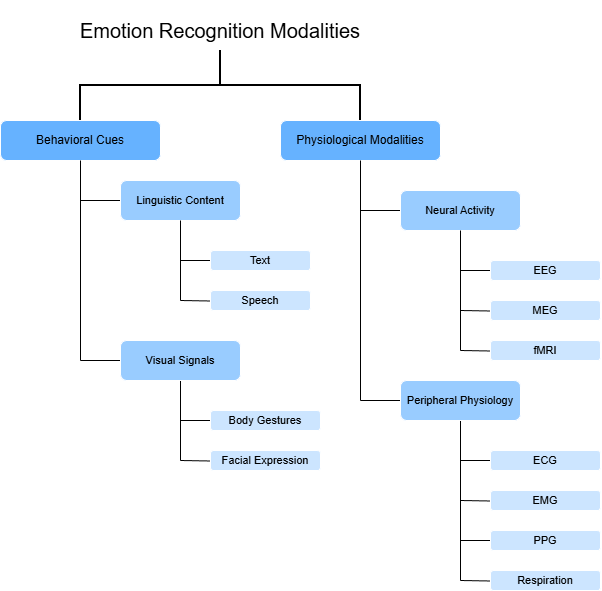
\includegraphics[width=0.5\linewidth]{pictures/Modalities.png}
    \caption{Modalities}
    \label{fig:modalities}
\end{figure}

Mittal et al. \cite{mittal2020m3er} have developed multimodal deep learning models that utilize attention mechanisms for modality contribution weightings depending upon their importance in a certain context, thus reducing the impact of unreliable modality contributions. Despite these models providing good contributions to this area by reducing the effects of unreliable contributions to a decision that is derived from a multimodal approach, they are still data-intensive optimization models that may not effectively succeed in the absence of available data. Priyasad et al. \cite{priyasad2020attention} have taken this concept a step further by developing attention-based models for multimodal fusion that have improved outcomes but are facing issues of model interpretability and increased computation.

The stability of affective patterns in multimodal datasets, such as in DEAP datasets, can improve emotion recognition according to Zheng et al., \cite{zheng2019stablepatterns}, although certain problems in bias and data modalities are still present. Similarly, Correa et al. \cite{correa2018amigos} employ AMIGOS multimodal data sets and are successful with subject-independent improvements, although large inter-subject variation in multimodal combinations remains a problem in achieving higher results in this area. From a review paper by Ma et al. \cite{ma2024peerjreview}, where certain improvements in the specified area are discussed, it’s noted that multimodal data sets are constantly more successful compared to their unimodal analogs and are working toward standardizing certain techniques in data evaluation.

Multimodal emotion modeling has been identified as a development that enhances the process of affective computing by incorporating EEG along with behavioral and physiological modalities to help computers effectively address the challenges that may come about due to the utilization of a single solution to the process. Although various fusion methods have been identified to have different advantages that may come in handy during the modeling process, they present various complexities, synchronicity considerations, or robustness during a fusion evaluation process. Multimodal models have been widely recognized for their incorporation of DL to increase adaptability to different forms of diverse modalities, which may come in handy during the decision process. Even though utilizing DL may demand extensive learning resources, various literature has been published to prove that the utilization of multimodal methods is significantly superior to the utilization of unimodal methods, as confirmed by literature focusing on various multimodal datasets such as DEAP, AMIGOS, MAHNOB-HCI, or MPED datasets. From the literature, multimodal methods have been recognized as a fundamental necessity for creating an effective EEG-based modeling approach suitable for operation in a realistic human-computer environment.

\subsection{EEG Correlates of Emotional States}
The essential basis of deriving emotion through an EEG remains rooted in the principle of recognizing the inherent rhythmic activity occurring over the human cortex as an outcome of the processing of emotion. It must also be noted here, unlike the conventional belief, the processing of an emotion is rarely indicated through the peak intensity of the EEG signal, as the expression of emotion largely remains indicated through a combination of dynamic activity occurring over a certain range of frequency bands. These, in turn, manifest as a product of the inherent neural activity underlying the emotion possessed by a particular individual \cite{geng2025dlreview}.

This view has driven emotion modeling from single-feature representations toward multiband, spatially distributed, and temporally evolving neural descriptions. The emerging evidence suggests that emotionality arises from the interaction of rhythmic modulation and interregional coordination, motivating feature extraction and representation strategies that explicitly capture frequency-specific activity, spatial asymmetries, and functional connectivity. 

Understanding the spectral and connectivity correlations for emotion is at the heart of how to develop efficient EEG-based emotion recognition systems. For example, frequency bands such as alpha have proved to have a certain level of consistency and subject stability of the scheme of emotions and therefore perform well to represent states of emotions for different subjects \cite{geng2025dlreview}. As a result, alpha bands have been deemed efficient for robust feature selection for subject-dependent and subject-independent emotion recognition systems.

Unlike alpha bands, the involvement of the beta band in emotional states, especially during heightened emotional states, is well evidenced, particularly in prefrontal regions, where a link to cognitive-emotional control parallels the involvement of arousal-related emotional regulation \cite{sun2022_db_dgcn_atffn}. In addition, delta and theta bands have been found to carry complementary information, with delta band activity related to emotional salience, while theta band connectivity is related to emotional integration/coordination \cite{zhang2023_multifreq_fc_emotion}.

More importantly, emotional states are also quantified through inter-channel correlations, where larger discriminability is observed, to obtain a holistic picture of neural interactions. Using these subspaces, finer quantification of emotional states is observed based on inter-channel correlation patterns, ensuring that a discriminative emotional state is quantified over localized band power features\cite{choong2021_corr_alpha_beta_gamma}. The time alignment effect is also observed to have an essential impact on neural components based on the emotional stimuli, reinforcing its importance in maintaining neural state changes in decision-making based on affect labeling\cite{liu2018_realtime_movie_induced}. Additionally, when basing research on interpretability, there is a need to quantify emotion based on significant patterns to avoid biases in the data set, leading to the wrong neural components \cite{qing2019_interpretable_eeg_emotion}.

Meanwhile, a comprehensive collection of research on EEG-based emotion recognition was conducted and summarized by Geng et al. \cite{geng2025dlreview}, during which the discussion focused on the characterization and importance of alpha activity when recognizing and understanding overall and general emotional dynamics and how sensitivity to emotion can benefit and possibly be enhanced through the exploration and investigation of other frequency bands, apart from the alpha band. A disadvantage and a possible drawback hidden in their discussion is the fact that these findings were summarized at a conceptual level. Sun et al. \cite{sun2022_db_dgcn_atffn} introduced the dual branch dynamic graph convolutional approach that directly addresses the beta-band activities, as well as the spatial relationships among the electrodes. This model proves that the emotional intensities, including the negative arousal, are indeed significantly detected in the modulation of the prefrontal beta signals. The process remains susceptible to cognition because the beta signals are also impacted by non-emotional cognitive activities. Zhang et al. \cite{zhang2023_multifreq_fc_emotion} proposed a multimodal functional connectivity approach that could simultaneously analyze delta, alpha, beta, and theta frequency bands. The results showed that there were significant emotion-related correlations in delta frequency bands and additional discriminative information from alpha and beta frequency bands.
In a study using the correlation-based approach for various frequency bands such as alpha, beta, and gamma frequency bands. The theta frequency band contributes mainly through the connectivity measures. The limitations of the study were the absence of explicit interaction modeling, which limited the value of the approach. Choong et al. \cite{choong2021_corr_alpha_beta_gamma} have attempted to investigate the use of correlations among alpha, beta, and gamma frequency band connectivity features and how the connectivity features under this use case have accounted for the identification of relevant emotional interactions, even when these interactions do not manifest as identifiable features across individual channels. Liu et al. \cite{liu2018_realtime_movie_induced} used movie-induced affective stimuli to retain the temporal traces of neural activities and provide time-aligned labels of affective states. While this method is effective for capturing dynamic responses related to emotions, it unfortunately depends highly on the inter-subject consistency in the perception of emotions, which may not generalize well to a truly diverse population or across different cultural contexts. Qing et al. \cite{qing2019_interpretable_eeg_emotion}, on the other hand, emphasized the aspect of model interpretability with the proposed mechanisms that connect the decision process with discernible patterns present in the signal. This enables a specific approach to validate that the underlying process utilizes neurophysiologically plausible features. However, the overall level of model interpretability is still hampered by the inherent complexity.

Collectively, this set of research supports the existence of a general neurophysiological framework for emotion states as encoded by both frequency-specific modulation, spatial organization, interregional connectivity, and even dynamics. Emotional states will be represented in the brain as an ensemble process of activity over multiple frequency bands and brain regions rather than as an expression of some global brain state. Clues provided by alpha and beta rhythms will be useful for both stability and intensity information, while salience and interregional integration will be provided by the delta and theta bands, with relational information provided by functional connectivity for differentiation among emotion states. Temporal dynamics and interpretability again increase the relative neurophysiological validity of emotion state representations to support EEG feature and modeling designs that well exceed local amplitude-based emotion recognition methods.

\subsection{EEG Signal Processing (Content to be humanized)}
EEG signal processing in emotion recognition aims to transform raw, noise-prone recordings into representations that preserve affect-relevant neurophysiological dynamics while remaining stable under inter-subject and inter-session variability. In practice, the signal-processing pipeline operates as a sequence of conditioning steps that (i) attenuate non-cerebral artifacts, (ii) standardize temporal structure for learning, and (iii) construct feature spaces that expose temporal, spectral, and spatial signatures of emotional states. This pipeline is not merely a front-end but a determinant of what information downstream models can exploit, and it directly shapes robustness, interpretability, and generalization.

Affective EEG is typically recorded under protocols in which emotional responses evolve across time, so processing must preserve transient changes (e.g., early perceptual responses) and sustained components (e.g., prolonged affective engagement). As datasets extend beyond strictly controlled laboratory environments, the pipeline increasingly emphasizes artifact resilience and cross-domain stability, motivating the integration of structured denoising, consistent segmentation, and multi-domain representations that align with modern deep learning encoders \cite{rahman2021eegreview}.

\subsection{Preprocessing}
Electroencephalogram signals are notoriously noisy and prone to various artifacts, so preprocessing is a crucial first step in EEG-based emotion recognition. This stage involves cleaning and transforming raw EEG data to improve its signal quality, remove or minimize artifacts, and standardize the inputs for subsequent feature extraction and classification. Effective preprocessing enhances the signal-to-noise ratio (SNR) of EEG by suppressing external interferences (e.g., power-line noise) and physiological artifacts (e.g., eye blinks, muscle movements), thereby boosting the performance of downstream emotion recognition models. Without adequate preprocessing, noise and artifacts can obscure the neural patterns related to emotions, leading to poor and unreliable classification results. It is therefore essential to apply carefully designed filtering, artifact removal, normalization, and other cleaning techniques before feature extraction. In addition, using consistent preprocessing protocols (e.g., the same filters and scaling across sessions or datasets) helps reduce variability and errors when comparing signals from different domains. Below, we review several key preprocessing methods and pipelines used in recent EEG-based emotion recognition studies, discussing their purposes, advantages, and limitations.

\subsubsection{Filtering and Noise Reduction}

Filtering and noise reduction form a foundational step in EEG signal preprocessing, aiming to clean the raw signals by eliminating various types of non-neural artifacts and retaining neurophysiologically relevant components. Given the sensitivity of EEG to external and internal noise sources, careful filtering is essential to ensure the signal reflects cognitive or affective brain activity rather than contamination from unrelated sources.

In the context of EEG-based emotion recognition, the importance of this step cannot be overstated. Emotional states are reflected in subtle variations within standard EEG frequency bands, such as delta ($\delta$), theta ($\theta$), alpha ($\alpha$), beta ($\beta$), and gamma ($\gamma$). However, these bands are easily overshadowed by artifacts such as low-frequency drifts (e.g., skin potentials or sweating), high-frequency muscle movements (EMG), and electrical interference (e.g., power-line noise). Without adequate filtering, these artifacts introduce variance that not only degrades classification performance but can also cause models to learn spurious correlations that lack neurophysiological validity.

Typical noise reduction approaches involve a combination of band-pass filtering to confine the signal within biologically meaningful frequency ranges, notch filtering to remove power-line interference (commonly at 50 or 60 Hz), and spatial filtering to reduce the impact of localized artifacts. More advanced strategies may also incorporate adaptive filtering techniques, such as regression-based correction using reference channels, or blind source separation to isolate and discard noise components. The choice of filter design—e.g., linear-phase FIR, Butterworth, or Chebyshev—plays a crucial role in avoiding phase distortion and preserving the temporal structure of emotional responses.

While these methods significantly improve the signal-to-noise ratio (SNR), they are not without challenges. Overly aggressive filtering can suppress genuine low- or high-frequency neural activity associated with emotion, leading to a loss of important affective information. Therefore, careful calibration and validation of filtering settings are required to balance noise suppression with the preservation of meaningful signal characteristics.

\subsubsection{Artifact Removal}

While filtering addresses many types of spectral noise in EEG, it is often insufficient to tackle non-stationary, physiological artifacts such as those caused by eye blinks, eye movements, facial muscles, and jaw tension. These artifacts can introduce abrupt, high-amplitude distortions that heavily contaminate the EEG signal, particularly in frontal and temporal regions—areas critical for affective processing. Thus, a dedicated artifact removal stage is essential to ensure that emotion-related brain activity is not masked by these extraneous signals.

In EEG-based emotion recognition, the need for robust artifact handling becomes more pronounced due to the fine-grained and often subtle nature of emotional state indicators in neural activity. A single blink or facial movement can produce amplitude spikes or frequency smearing that overwhelm the weaker emotional signatures in the data. Furthermore, because emotional elicitation often involves visual or auditory stimuli, the likelihood of such artifacts increases during experimental protocols.

Artifact removal techniques typically aim to isolate and suppress these non-neural components without discarding meaningful brain signals. Blind source separation methods, such as Independent Component Analysis (ICA), are commonly employed to decompose EEG into statistically independent components. Once separated, components suspected of containing artifacts can be attenuated or excluded. Other strategies involve regression-based correction using auxiliary channels (e.g., EOG), spatial filtering techniques that emphasize cortical over peripheral sources, or machine learning models trained to detect artifact patterns.

Although effective in enhancing signal clarity, artifact removal methods face limitations such as subjectivity in manual component identification, potential loss of neural information, and computational cost in real-time settings. These challenges have prompted research into automated and hybrid approaches that can balance artifact suppression with signal preservation, particularly for emotion-related applications where data quality is paramount.

\subsubsection{Hybrid ICA-Wavelet Techniques}

While standalone artifact removal methods such as ICA or wavelet filtering can effectively suppress certain types of noise in EEG, combining these approaches often yields superior results. Hybrid ICA-wavelet techniques have gained attention for their ability to blend spatial decomposition and time-frequency analysis, offering a more adaptive and precise strategy for cleaning EEG signals.

In the context of emotion recognition, where neural patterns linked to affective states are subtle and susceptible to corruption by eye blinks, muscle movements, and environmental noise, these hybrid techniques are especially valuable. They provide a pathway to remove artifacts without significantly compromising the emotional content encoded in neural activity. As EEG-based affective computing systems move toward higher sensitivity and broader deployment, the ability to automatically and selectively clean physiological noise becomes increasingly important.

Broadly, hybrid ICA-wavelet approaches begin by decomposing EEG data into statistically independent components, enabling separation of neural and non-neural sources. Rather than removing entire components identified as noisy—which can risk discarding useful brain signals—wavelet analysis is then applied to these components to isolate and suppress the specific temporal or spectral segments associated with artifacts. The cleaned signals are subsequently reconstructed, preserving genuine neural activity while minimizing contamination. These techniques balance spatial unmixing with targeted temporal filtering, making them well-suited to complex, real-world EEG data.

Despite their promise, hybrid methods come with trade-offs. They require careful parameter tuning and can be computationally intensive. Moreover, their effectiveness may vary depending on the type and severity of artifacts present, as well as the chosen wavelet functions or decomposition levels. Nevertheless, their demonstrated impact on improving classification performance in EEG emotion recognition systems highlights their potential as an advanced preprocessing strategy.

\subsubsection{Channel Selection and Spatial Filtering}

Channel selection and spatial filtering represent fundamental preprocessing strategies aimed at enhancing signal quality by optimizing how EEG data is spatially represented. Instead of treating all electrodes equally, these techniques emphasize the most informative regions of the scalp while mitigating contributions from noisy or irrelevant channels. This is particularly critical for EEG-based emotion recognition, where subtle affective signals are often localized and easily masked by extraneous neural or physiological activity.

In affective computing, focusing on emotionally salient brain regions—such as the prefrontal and temporal areas—has proven effective in improving classification performance. Selecting a targeted subset of electrodes reduces data dimensionality, minimizes the influence of noise-prone channels, and simplifies the computational pipeline. Spatial filtering, on the other hand, enhances signal clarity by re-referencing EEG data to remove global noise components, thereby amplifying localized neural patterns relevant to emotional states.

Various strategies are employed in practice. Manual or data-driven channel selection methods prioritize electrodes based on prior neuroscientific knowledge or feature contribution metrics, ensuring that only the most discriminative channels are retained. Spatial filters such as the common average reference (CAR) and Laplacian filtering are widely used to reduce reference bias and suppress common-mode noise. These filters help normalize EEG input across channels and reveal spatial gradients that may correlate with affective processes.

Although these methods offer practical advantages—including reduced computational load and improved robustness—they also introduce trade-offs. Excessive channel reduction may eliminate distributed emotional signals, and spatial filters can sometimes distort signal topographies if improperly applied. Hence, careful consideration of the recording setup and application context is essential when designing preprocessing pipelines around spatial structure.


\renewcommand{\arraystretch}{1.2}
\setlength{\tabcolsep}{5pt}
\begin{small}
\begin{longtable}{
>{\raggedright\arraybackslash}p{0.13\textwidth}
>{\raggedright\arraybackslash}p{0.22\textwidth}
>{\raggedright\arraybackslash}p{0.18\textwidth}
>{\raggedright\arraybackslash}p{0.20\textwidth}
>{\raggedright\arraybackslash}p{0.22\textwidth}
}
\caption{Representative studies on EEG preprocessing techniques for emotion recognition.}
\label{tab:eeg_preprocessing_summary} \\

\toprule
\textbf{Study} & \textbf{Approach} & \textbf{Advantages} & \textbf{Limitations} & \textbf{Key Findings} \\
\midrule
\endfirsthead

\multicolumn{5}{c}{\textit{Table~\ref{tab:eeg_preprocessing_summary} continued}} \\
\toprule
\textbf{Study} & \textbf{Approach} & \textbf{Advantages} & \textbf{Limitations} & \textbf{Key Findings} \\
\midrule
\endhead

\midrule
\multicolumn{5}{r}{\textit{Continued on next page}} \\
\endfoot

\bottomrule
\endlastfoot

Somers \textit{et al.}~\cite{somers2018mcwfilter} & Multi-channel Wiener filtering for artifact suppression & Preserves neural signal while reducing ocular/muscle noise & Needs covariance estimates; less effective for nonstationary noise & Improves EEG signal quality before emotion decoding \\

Kang \textit{et al.}~\cite{kang2019_ica_aug} & ICA with heuristic artifact-aware rejection & Effectively isolates and removes major EEG artifacts & Manual component selection may reduce reproducibility & Boosts classification accuracy post-cleaning \\

Phadikar \textit{et al.}~\cite{sphadi2021automati} & Wavelet thresholding for blink artifact removal & Fast and adaptive for blink noise & Limited to blink artifacts; not general-purpose & Strengthens EEG robustness in emotion pipelines \\

Koelstra \textit{et al.}~\cite{Koelstra2012} & Bandpass filtering with baseline normalization & Reduces noise and inter-subject variability & Requires baseline segment; may remove useful bands & Improves single-trial emotion classification \\

Mahajan \& Morshed~\cite{Mahajan2014} & Wavelet-enhanced ICA artifact removal & Automated ocular artifact suppression & Mainly targets eye-blink artifacts & Enhances EEG quality for emotion analysis \\

Val-Calvo \textit{et al.}~\cite{ValCalvo2019} & Lightweight real-time preprocessing pipeline & Low-latency and computationally efficient & Simplified features limit generalization & Enables real-time EEG emotion recognition \\

\end{longtable}
\end{small}



\subsubsection{Feature Extraction}
Feature extraction maps preprocessed EEG into representations that make emotion-related patterns more separable. The dominant organizing principle is that affective neural responses manifest jointly in time, frequency, and scalp space; therefore, emotion-relevant information is rarely captured by a single domain alone. Feature extraction strategies can be broadly viewed as (i) explicit, signal-derived representations (e.g., temporal statistics, spectral summaries, and time-frequency maps) and (ii) learned representations, where deep models infer discriminative structure directly from minimally processed EEG or from engineered inputs.

A major practical trend is the construction of structured, model-friendly tensors that preserve multi-domain dependencies. Instead of producing isolated scalar features per channel, pipelines increasingly generate 2D or 3D objects (e.g., channel $\times$ time, channel $\times$ frequency, or time $\times$ frequency maps per channel) so that convolutional encoders can exploit locality and compositional structure. A related direction uses 3D feature representations paired with fully convolutional models, which treat temporal-spatial-spectral structure as a unified object, reducing the need for manual fusion and allowing end-to-end learning of cross-domain interactions \cite{li2021_3dfeatdfcn}.

Sequential feature formation is also prominent because emotional responses evolve over time. Spatial-temporal representations can be formed by stacking window-level descriptors and then applying sequence models such as bidirectional recurrent units to capture temporal dependencies across windows. This approach preserves local temporal detail while modeling longer-range affective trajectories, which is useful when emotional episodes unfold gradually rather than changing abruptly \cite{lew2020bigruspatiotemporal}.

Also, transformer-aided feature learning improves cross-domain modeling, as it provides attention-driven integration across time and channels. Conformer-like architectures, which include convolution to detect local patterns as well as transformer attention to uncover global interdependencies, give a useful tool to encode EEG signals as local patterns or global connections not relying on manually defined fusion strategies \cite{song2022eegconformer}. Also, models based on parallel transformers and 3D convolution adhere to the same principle, according to which transformers are responsible for capturing interdependencies, while 3D convolution is responsible for capturing structurally well-defined spatiotemporal links related to Emotion concepts \cite{sun2022paralleltransformer3dcnn}.

Many EEG-based emotion recognition methods rely on frequency-domain features derived from the preprocessed signals. For example, power spectral density (PSD) and differential entropy (DE) features are among the most commonly used representations of EEG in emotion studies. PSD features capture the distribution of signal power across standard frequency bands (theta, alpha, beta, etc.), summarizing how much rhythmic activity is present in each band during an emotional state. Differential entropy is a closely related measure: if we assume the EEG amplitude in a short time window follows a Gaussian distribution, the differential entropy $h$ of that signal is given by 
\begin{equation}
    h = \frac{1}{2}\ln(2\pi e,\sigma^2), 
\end{equation}
where $\sigma^2$ is the signal’s variance. Because variance is proportional to signal power in the window, DE is essentially a log-power feature. In practice, computing DE for an EEG segment yields a value that increases with the signal’s power in that segment and is often taken band-wise (so DE in delta, theta, etc. can be calculated similarly to band power).

Power spectral density (PSD) and differential entropy (DE) features are widely adopted in EEG-based emotion recognition because they effectively capture the frequency-domain characteristics of brain activity linked to emotional processing. DE, in particular, is often preferred over raw power features due to its improved numerical stability and better alignment with Gaussian assumptions, making it more suitable for common classifiers. These spectral features are typically computed over defined EEG bands (such as delta, theta, alpha, beta, and gamma), offering compact, fixed-length representations that are easy to integrate into machine learning models. One of the key advantages of using PSD or DE is their robustness to temporal misalignment across trials, since they summarize amplitude-based energy without relying on phase information. Additionally, after appropriate filtering, these features are relatively resistant to high-frequency noise. However, because they average power over time windows, they may discard valuable temporal dynamics that unfold across shorter intervals, which can be important for tracking affective shifts. There's also the assumption of signal stationarity within each segment, which can be problematic if emotional states evolve non-uniformly during stimulus presentation. To address these concerns, the choice of window size, overlap, and frequency resolution must be tuned carefully to balance temporal sensitivity with spectral precision. Despite these trade-offs, PSD and DE remain foundational tools in affective EEG research, serving as reliable baselines and often informing the design of more complex models.

In summary, preprocessing is an indispensable component of EEG-based emotion recognition that directly impacts the reliability of the results. Across the literature, there is a clear trend toward more sophisticated and automated preprocessing pipelines. Early studies relied on simple filtering and manual artifact rejection, but recent works (including those reviewed above) employ advanced techniques like ICA-based cleaning, wavelet denoising, and automated channel selection to obtain cleaner EEG signals. The overarching insight is that improving signal quality upstream yields significant gains in model performance downstream. Another trend is an emphasis on standardization and consistency in preprocessing—researchers ensure that data from different subjects, sessions, or datasets undergo the same filtering, normalization, and feature extraction procedures, which is crucial for generalizable models. As EEG emotion datasets grow and real-world applications demand online analysis, preprocessing methods are moving toward real-time-capable implementations (e.g., using adaptive filters or on-the-fly ICA updates) and minimizing the need for human intervention. In the coming years, we expect preprocessing to continue evolving with the integration of novel signal processing techniques (for example, deep-learning-based artifact correction) to enhance the quality of EEG data further. Such developments will strengthen the foundation for accurate and robust emotion recognition from brain signals, as even the most powerful classification algorithm can only be as good as the data it receives.

\paragraph{Temporal, Frequency, and Spatial Feature Concepts \& Cross-Domain Feature Fusion}
Electroencephalography (EEG) signals intrinsically span multiple domains: temporal, frequency, and spatial. Each captures unique characteristics of brain activity. Temporal-domain features reflect the dynamic evolution of neural responses over time, often extracted by segmenting EEG signals into time windows or leveraging time-series analyses (e.g., using sliding windows to capture transient patterns). Frequency-domain features are obtained by transforming EEG signals (e.g. via Fourier transform) to reveal power in canonical frequency bands (δ: 1–3 Hz, θ: 4–7 Hz, α: 8–13 Hz, β: 14–30 Hz, γ: 30–50 Hz). Notably, different frequency bands carry distinct emotional significance—for example, prior studies have found that certain bands (e.g., beta, gamma) respond more strongly to specific emotional stimuli. A common frequency feature is differential entropy (DE), defined for a signal (modeled as Gaussian) as:
\begin{equation}
H(X) = \frac{1}{2}\ln\left(2\pi e\,\sigma_X^2\right)
\end{equation}
where $\sigma_X^2$ is the signal variance in a given band. DE features in multiple bands provide a compact spectrum representation for emotion recognition. Spatial features encode the distribution of EEG activity across brain regions and electrodes. For instance, one can compute an inter-channel correlation matrix $R$ to quantify functional connectivity: each entry can be the Pearson correlation $r_{ij}$ between channels $i$ and $j$,
\begin{equation}
r_{ij} = \frac{\operatorname{Cov}(x_i, x_j)}{\sqrt{\operatorname{Var}(x_i)\operatorname{Var}(x_j)}}
\end{equation}
yielding an adjacency matrix for graph-based spatial representations. In summary, EEG data provide multi-domain information: temporal dynamics, spectral content, and spatial patterns across the cortex. These domains are often referred to as multi-domain features, and leveraging all three can give a more holistic view of the underlying emotional state.

\begin{figure}
    \centering
    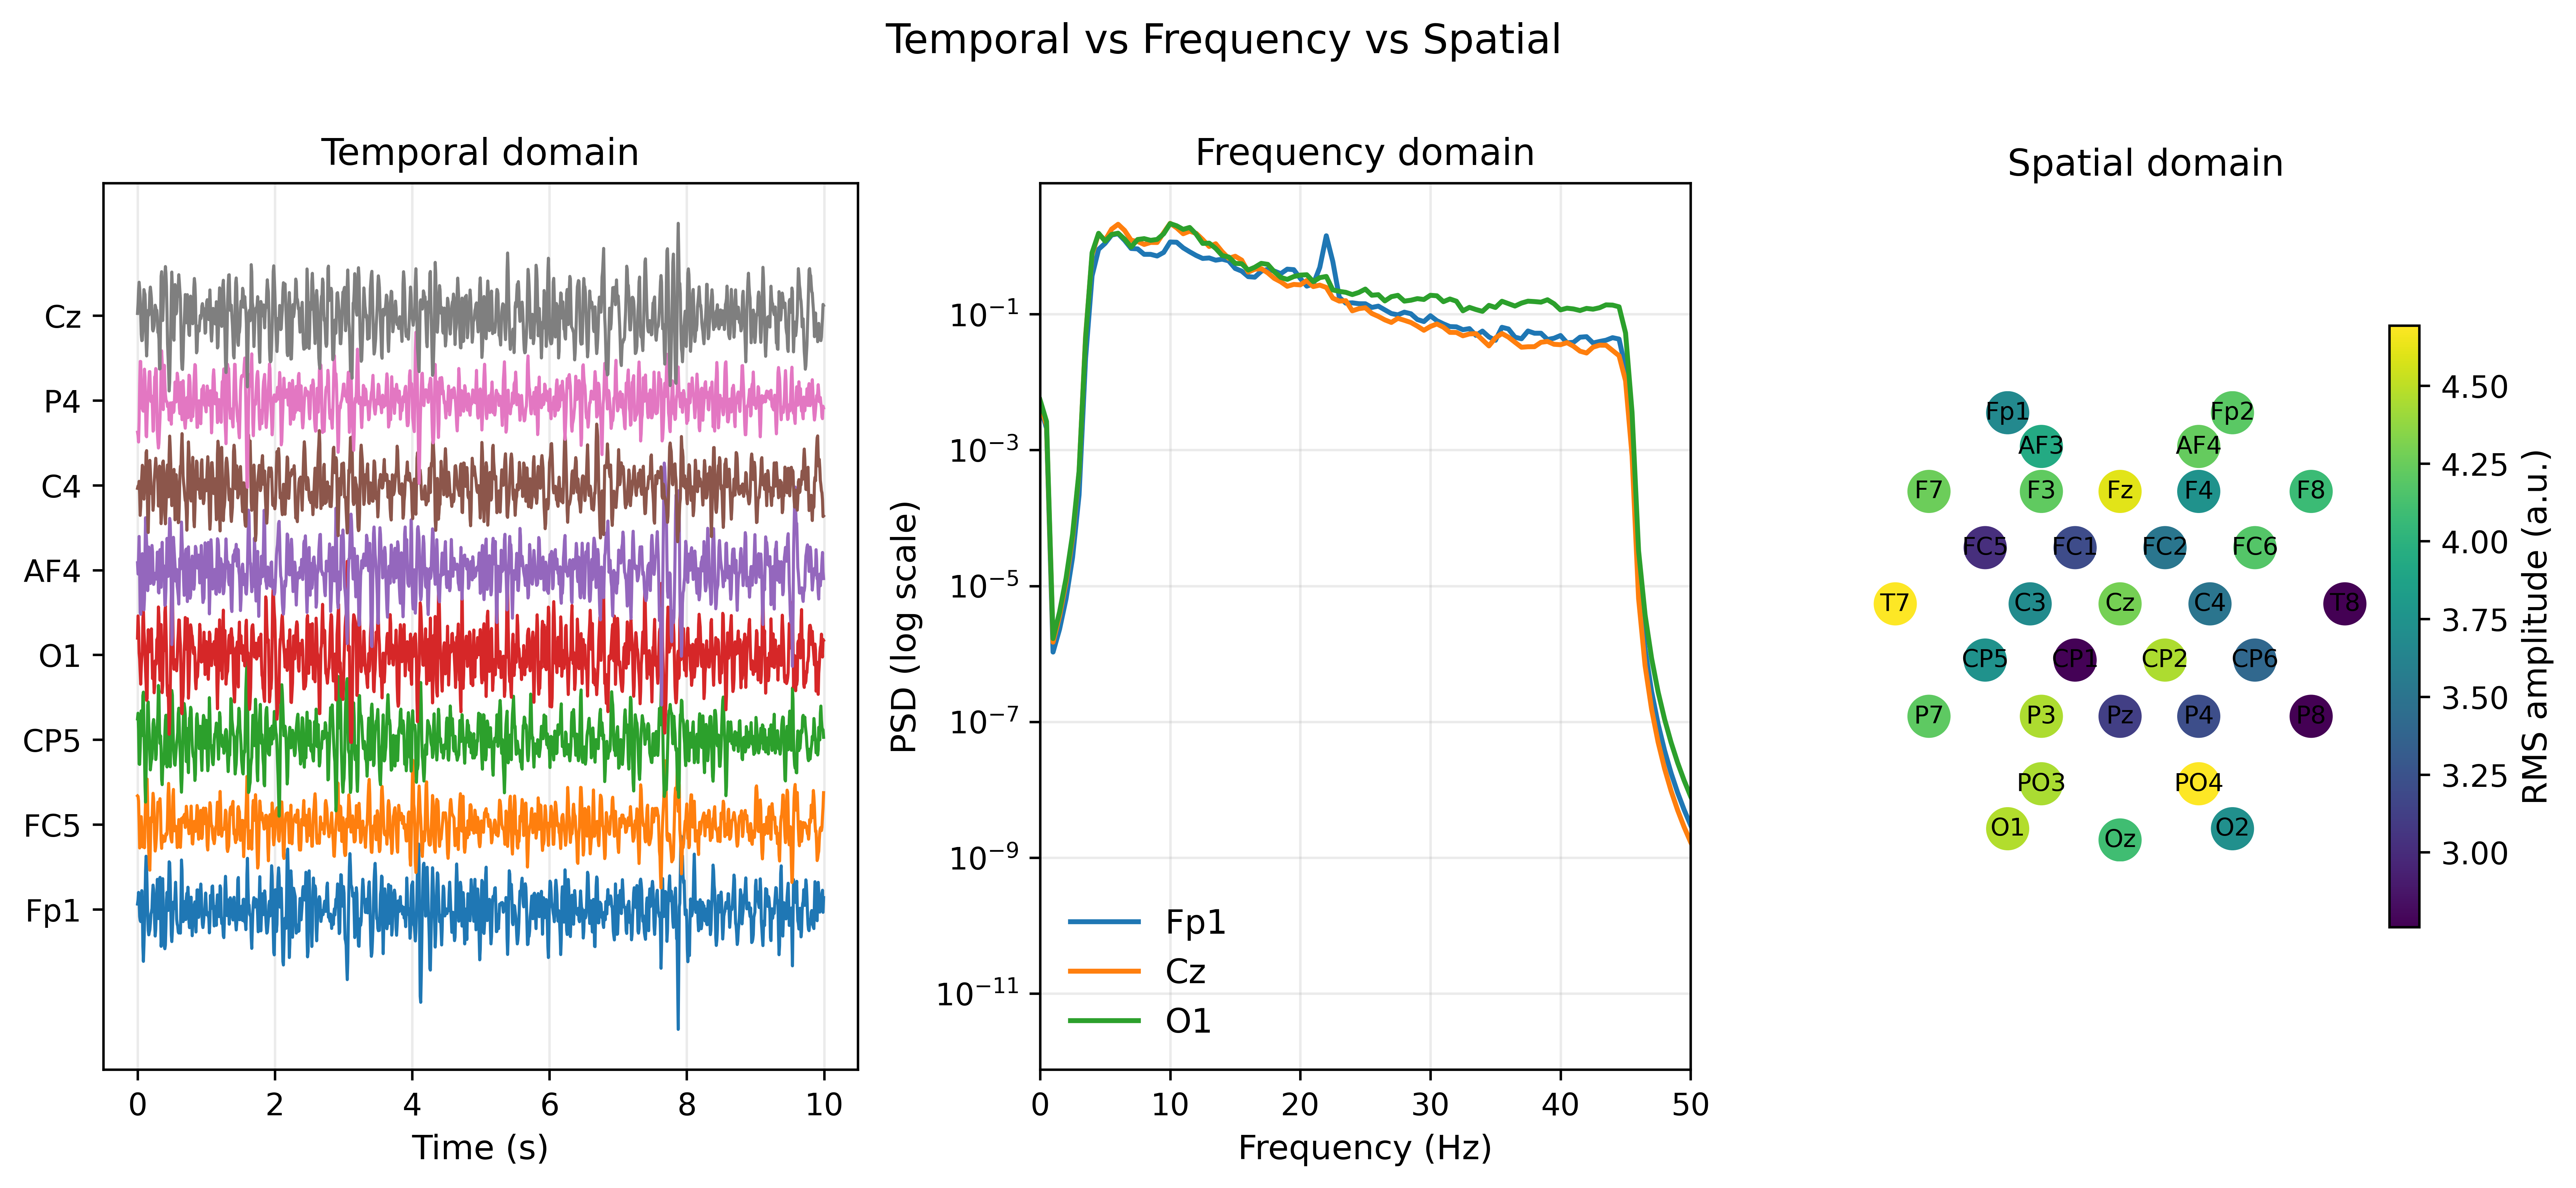
\includegraphics[width=0.75\linewidth]{pictures/tem_freq_spa.png}
    \caption{Temporal vs Frequency vs Spatial Domain}
    \label{fig:temp_freq_spatial}
\end{figure}

Each domain contributes complementary information for recognizing emotions from EEG, and fusing them leads to more robust and accurate models. Temporal features capture how emotional responses unfold and vary, which is crucial since emotions are inherently time-dependent processes (for example, the rise and fall of arousal levels in response to a stimulus). Frequency features isolate activity in neurophysiological bands linked to affective processes—for instance, changes in alpha or beta power can indicate relaxation or heightened engagement, respectively. Spatial features localize emotional processing to particular brain regions (e.g., frontal asymmetry in the alpha band is a known correlate of affective valence). Because these aspects are complementary, integrating them can compensate for the weaknesses of any single feature type. Empirical results have shown that models using combined temporal–spectral–spatial representations outperform those using one domain alone. In particular, spatial features are often paired with temporal or frequency features to provide context to where in the brain certain temporal or spectral patterns occur. The fusion of multi-domain features thus yields a richer representation of the EEG: it can improve emotion recognition accuracy and robustness to noise or variability. Overall, leveraging all three domains helps capture the full spectrum of EEG correlates of emotion, enabling models to generalize better across subjects and conditions.

Fusion is implemented through multiple architectural patterns. First, \emph{tensor fusion} constructs multi-dimensional inputs (e.g., 3D stacks) so that a single encoder learns interactions implicitly by operating on structured volumes. Second, \emph{multi-branch fusion} assigns specialized encoders to each domain (temporal, spectral, and spatial) and then merges intermediate embeddings. Third, \emph{attention-based fusion} uses learned gates or attention weights to adaptively emphasize the most informative domain or channel subsets under changing noise conditions. A dual-branch dynamic graph convolution combined with adaptive transformer fusion illustrates how graph-based spatial reasoning and attention-driven integration can be combined to exploit inter-channel structure while remaining flexible in weighting features across domains \cite{sun2022atffnet}. For explicitly multi-domain EEG encodings, transformer networks are also designed to ingest representations from multiple feature spaces and integrate them through attention, encouraging stable fusion under heterogeneous recording conditions \cite{sun2023meegtransformer}.

\subparagraph{Temporal Domain Features:}
Temporal-domain features are essential in EEG-based emotion recognition due to the inherently dynamic nature of affective experiences. Emotions unfold over time, often manifesting as a sequence of neural events that cannot be fully captured by static or time-agnostic features. Temporal representations enable models to interpret how brain activity evolves in response to emotional stimuli, capturing transitions between emotional states, momentary peaks of affect, or sustained emotional engagement. These features are particularly important for dealing with inter-subject variability in the timing of emotional responses, as they allow the model to focus on temporal signatures rather than relying solely on synchronized stimuli or labels.

In the context of emotion decoding, temporal modeling has been integrated using various deep learning strategies that exploit sequence learning capabilities. For instance, recurrent models such as LSTMs or bidirectional RNNs have been commonly employed to extract dependencies across consecutive EEG segments, learning how affective states change over time. Some hybrid approaches combine convolutional layers with recurrent units to capture both spatial patterns and their temporal evolution. Other models use hierarchical sequence architectures that process signals regionally before integrating them globally, preserving spatial structure while extracting dynamic trajectories. Additionally, temporal convolutional architectures have emerged as an alternative to RNNs, enabling efficient modeling of long-range dependencies through layered, dilated convolutions.

While these methods improve the ability to recognize dynamic emotional patterns, they often face challenges such as limited integration with frequency and spatial information or assumptions about uniform timing across trials. Selecting appropriate window lengths and temporal resolution remains crucial to ensure relevant patterns are captured without losing detail or overfitting. Nonetheless, temporal-domain modeling remains a cornerstone in enhancing emotion recognition performance, especially in naturalistic or continuous affective scenarios where the timing of emotional expression varies significantly across individuals.

\subparagraph{Frequency Domain Features:}
Frequency-domain features are essential for extracting the oscillatory characteristics of EEG signals that correlate with emotional processes. Changes in alpha, beta, theta, and gamma band power reflect arousal and valence dimensions. These rhythms provide stable indicators across sessions and individuals when appropriately filtered.
Li et al.~\cite{li2021multidomain} proposed a multi-domain adaptive graph convolutional network that integrated temporal and DE-based frequency features using dual-channel correlation graphs. By extracting frequency information separately and fusing it with temporal dependencies, the model improved recognition performance. Its limitation lies in the reliance on prototype-guided adjacency matrices that may reduce generalizability. Song et al.~\cite{song2022eegconformer} introduced EEG-Conformer, combining convolution and Transformer-based attention to encode temporal and frequency features jointly. Frequency-domain inputs were processed as patch-level spectral tokens. This model achieved state-of-the-art performance, but careful regularization was needed to prevent overfitting due to high model capacity. Zheng et al.~\cite{zheng2022multi} used short-time Fourier transform (STFT)-based spectrogram features for EEG emotion classification and applied deep CNNs to learn frequency-band contributions. The approach benefited from explicit band decomposition but was sensitive to STFT parameter settings.
Frequency-domain methods highlight emotion-related rhythmic activity and are crucial for distinguishing affective responses. Effective designs often combine frequency with other domains, though pure frequency-based models risk missing temporal structure. Limitations include parameter sensitivity, generalization to unseen individuals, and interpretability of spectral features.

\subparagraph{Temporal-Frequency Domain Features:}
Frequency-domain features are a cornerstone in EEG-based emotion recognition, as they capture the rhythmic patterns of brain activity that are closely tied to emotional processing. Oscillations within specific frequency bands—such as delta (1–4 Hz), theta (4–8 Hz), alpha (8–13 Hz), beta (13–30 Hz), and gamma (30–50+ Hz)—have been shown to reflect various aspects of affective states. For example, changes in alpha and beta power are commonly linked to arousal and valence, with frontal alpha asymmetry often associated with approach–withdrawal tendencies. These frequency-specific modulations are generally stable across sessions and subjects, making them reliable indicators for emotion classification.

In practical systems, frequency-domain analysis typically involves transforming the EEG time series using tools such as the Fourier transform, wavelet decomposition, or differential entropy computation. These transformations yield compact representations that emphasize oscillatory energy in targeted bands, often aggregated over time windows. This abstraction allows models to focus on spectral patterns rather than the raw signal, which is more susceptible to noise and temporal misalignment.

Recent modeling strategies incorporate frequency-domain features in various ways. Some architectures extract frequency features independently and fuse them with temporal or spatial representations to enrich emotion-specific information. Others use convolutional or attention-based encoders to process spectrograms or patch-based frequency representations, treating them as visual inputs to learn high-level spectral abstractions. There are also approaches that apply graph-based reasoning on frequency-encoded nodes to uncover inter-band relationships and regional dynamics.

Despite their strength, frequency-domain methods come with trade-offs. Their performance can be sensitive to the choice of decomposition parameters and windowing strategies. Models that focus solely on spectral information may overlook important temporal dynamics or fail to adapt across subjects with varying spectral profiles. Nevertheless, when combined effectively with other modalities, frequency-domain features offer robust insight into the oscillatory structure of affective brain states and significantly enhance emotion recognition systems.

\subparagraph{Integration and Fusion Strategies Across Feature Domains:}
Integrating temporal, frequency, and spatial features has become a central focus in EEG-based emotion recognition due to the inherently multidimensional nature of affective brain responses. Each domain captures different but complementary aspects of emotional processing—temporal features track the evolution of neural activity, frequency features reflect oscillatory signatures, and spatial features map activity across brain regions. Emotion expression in the brain does not reside in isolated channels or bands but emerges from interactions across these domains. Therefore, holistic representations that combine these views are more expressive and tend to offer better generalization across subjects and sessions.

Multi-domain fusion is particularly important when dealing with noisy or variable EEG data. One domain may be less informative or more corrupted in certain conditions (e.g., noisy temporal dynamics due to movement), but combining signals from multiple domains allows the model to fall back on more reliable representations. This redundancy makes fusion strategies more robust, especially for real-world and cross-subject applications.

Recent advances in multi-domain fusion architectures have emphasized flexibility and adaptiveness. Many approaches employ multi-branch designs where domain-specific feature extractors process temporal, spectral, and spatial signals in parallel, followed by fusion layers that merge the representations. Some use graph convolutional networks (GCNs) to model spatial relationships between EEG channels and combine these with temporal-frequency encoders. Others introduce attention-based mechanisms that learn to weigh features across domains dynamically based on their relevance to the emotional state, enabling adaptive and context-sensitive fusion.

There is also a shift toward deep models that learn fusion strategies implicitly, rather than relying on manually designed combinations. These include transformer-based encoders with domain-specific attention heads and masked modeling strategies for cross-domain reconstruction. Such models are powerful but typically computationally intensive, requiring large memory resources and careful regularization to avoid overfitting. Additionally, they raise questions about interpretability—understanding how different domains contribute to emotion prediction remains a challenge.

In summary, integrating multiple EEG domains enhances the model’s ability to learn discriminative and generalizable emotion representations. Fusion methods allow for richer modeling of affective patterns, better handling of noise, and more stable cross-subject performance. While these strategies offer significant benefits, they must be carefully balanced to manage computational complexity and ensure that models remain interpretable and adaptable across contexts. Future research is likely to focus on more lightweight, interpretable, and data-efficient fusion techniques that preserve the advantages of multi-domain integration while being practical for real-time applications.

\renewcommand{\arraystretch}{1.2}
\setlength{\tabcolsep}{5pt}
\begin{small}
\begin{longtable}{
>{\raggedright\arraybackslash}p{0.13\textwidth}
>{\raggedright\arraybackslash}p{0.22\textwidth}
>{\raggedright\arraybackslash}p{0.18\textwidth}
>{\raggedright\arraybackslash}p{0.20\textwidth}
>{\raggedright\arraybackslash}p{0.22\textwidth}
}
\caption{Representative studies on EEG feature extraction techniques for emotion recognition.}
\label{tab:eeg_feature_extraction_summary} \\

\toprule
\textbf{Study} & \textbf{Approach} & \textbf{Advantages} & \textbf{Limitations} & \textbf{Key Findings} \\
\midrule
\endfirsthead

\multicolumn{5}{c}{\textit{Table~\ref{tab:eeg_feature_extraction_summary} continued}} \\
\toprule
\textbf{Study} & \textbf{Approach} & \textbf{Advantages} & \textbf{Limitations} & \textbf{Key Findings} \\
\midrule
\endhead

\midrule
\multicolumn{5}{r}{\textit{Continued on next page}} \\
\endfoot

\bottomrule
\endlastfoot

Li \textit{et al.}~\cite{li2021_3dfeatdfcn} & 3D spatial-temporal-spectral features with FCNs & Combines rich domain information in unified volume & Heavier computation than 2D encodings & Improves accuracy across datasets \\

Lew \textit{et al.}~\cite{lew2020bigruspatiotemporal} & Spatiotemporal encoding with Bi-GRU & Captures evolving emotion responses & Sensitive to segmentation granularity & Better for gradual emotion transitions \\

Song \textit{et al.}~\cite{song2022eegconformer} & Conformer model for EEG sequences & Fuses local and global patterns effectively & Can overfit without regularization & Outperforms traditional CNN/RNN models \\

Jia \textit{et al.}~\cite{jia2020sstemotionnet} & 3D DenseNet with attention across domains & Learns dynamic relevance between features & Model complexity is high & Salient EEG areas enhance emotion decoding \\

Sun \textit{et al.}~\cite{sun2022paralleltransformer3dcnn} & Parallel transformer + 3D CNN fusion & Separates local/global representation branches & Careful tuning required for balance & Shows strong performance on multi-channel inputs \\

Yudhana \textit{et al.}~\cite{yudhana2020human} & FFT-based spectral features with $k$NN classifier & Simple and computationally efficient & Ignores temporal dynamics; limited scalability & Shows the viability of classic frequency features \\

Chen \textit{et al.}~\cite{chen2019feature} & Differential entropy features with LDA projection & Compact and discriminative spectral representation & Linear assumptions limit expressiveness & Improves valence and arousal classification \\

Bigirimana \textit{et al.}~\cite{bigirimana2020emotion} & Multi-class CSP spatial filtering & Enhances emotion-specific spatial patterns & Sensitive to non-stationarity and subject variation & Boosts multi-class EEG emotion accuracy \\

\end{longtable}
\end{small}

\subsection{Feature Selection}
Electroencephalogram (EEG) emotion datasets often contain high-dimensional feature vectors (e.g., numerous channels and frequency-band features), while sample sizes are relatively limited. This disparity can lead to the curse of dimensionality and model overfitting, where irrelevant or redundant features degrade generalization performance. Feature selection addresses this by reducing the feature space to only the most informative and non-redundant features, thus improving classifier training efficiency and robustness. In EEG-based emotion recognition, selecting a compact set of relevant features (or channels) has been shown to improve classification accuracy and stability across subjects. For example, removing noisy channels/features can boost signal-to-noise ratio and emotion recognition performance. Overall, an effective feature selection step can enhance prediction accuracy, reduce model complexity, and facilitate easier interpretation of the brain patterns underlying emotions~\cite{hamzah2024heliyon}.

\subsubsection{Filter Methods}
Filter-based feature selection is a widely used approach in EEG-based emotion recognition due to its simplicity, speed, and model-agnostic nature. These methods assess the importance of features using statistical or information-theoretic metrics before the training of any classification model. As a result, they are often applied as a preliminary step in the machine learning pipeline to reduce dimensionality and improve the learning efficiency of downstream classifiers.

The relevance of this subsubsection lies in the high-dimensional and noisy nature of EEG data. Emotion-related signals are often embedded within a larger pool of redundant or irrelevant features. By filtering out less informative features early in the pipeline, filter methods help improve classification performance, reduce overfitting, and enhance interpretability. This is especially critical in EEG emotion recognition, where datasets are often limited in size but rich in feature complexity.

Several techniques are commonly used in filter-based selection. Correlation-based methods assess the linear relationship between individual features and the emotion labels, promoting features that show strong dependency with the target class. Mutual information (MI)-based approaches evaluate both the relevance of a feature to the emotion label and its redundancy with other features. This balance is the core of the Minimum Redundancy Maximum Relevance (mRMR) framework, which aims to select a compact, non-redundant subset of features that are highly informative. Extensions of this idea incorporate search strategies like sequential forward or floating selection to explore the feature space more thoroughly while maintaining efficiency.

Despite their strengths, filter methods have limitations. They typically ignore feature interactions since features are ranked independently. This can lead to suboptimal subsets when emotional patterns are distributed across combinations of features rather than isolated ones. Moreover, the selected features may not align with the optimal decision boundaries of specific classifiers, which can affect model performance in some cases. Nevertheless, due to their scalability and general applicability, filter methods remain a valuable component of EEG emotion recognition systems.

\subsubsection{Wrapper Methods}
Wrapper-based feature selection represents a powerful yet computationally demanding strategy for identifying the most informative EEG features in emotion recognition tasks. Unlike filter methods, which evaluate features independently of any model, wrappers directly incorporate a learning algorithm into the selection process. This allows them to assess how different feature subsets perform in actual classification scenarios, resulting in more tailored and often higher-performing feature sets.

The importance of wrapper methods in EEG emotion recognition stems from their capacity to consider complex feature interactions and nonlinear relationships that are often present in affective EEG data. Since emotional responses can be subtle and involve coordinated changes across multiple brain regions and frequency bands, capturing these interdependencies is essential. Wrappers are particularly useful in this context because they evaluate combinations of features holistically, optimizing subsets for performance with a given classifier.

Several techniques exemplify the wrapper approach. Recursive Feature Elimination (RFE) is a classic method that systematically removes the least useful features based on classifier weights or accuracy impact, refining the subset over iterations. Evolutionary strategies like genetic algorithms and differential evolution have gained popularity for exploring the large EEG feature space efficiently. These approaches iteratively evolve candidate feature sets by simulating biological processes such as mutation, selection, and crossover, guided by model validation performance. Such methods can yield highly optimized feature combinations that enhance classification accuracy and generalization across subjects.

However, wrapper methods come with challenges. Their reliance on repeated model training makes them computationally expensive, especially when the feature set is large or the classifier is complex. This can limit their practicality in real-time or resource-constrained environments. Additionally, overfitting can occur if the evaluation criterion is not carefully regularized or if the feature selection process is too tightly coupled to a specific dataset. Despite these drawbacks, wrapper-based methods remain valuable tools for discovering high-quality feature subsets that boost emotion recognition performance in EEG applications.


\renewcommand{\arraystretch}{1.2}
\setlength{\tabcolsep}{5pt}
\begin{small}
\begin{longtable}{
>{\raggedright\arraybackslash}p{0.13\textwidth}
>{\raggedright\arraybackslash}p{0.22\textwidth}
>{\raggedright\arraybackslash}p{0.18\textwidth}
>{\raggedright\arraybackslash}p{0.20\textwidth}
>{\raggedright\arraybackslash}p{0.22\textwidth}
}
\caption{Representative studies on EEG feature selection techniques for emotion recognition.}
\label{tab:eeg_feature_selection_summary} \\

\toprule
\textbf{Study} & \textbf{Approach} & \textbf{Advantages} & \textbf{Limitations} & \textbf{Key Findings} \\
\midrule
\endfirsthead

\multicolumn{5}{c}{\textit{Table~\ref{tab:eeg_feature_selection_summary} continued}} \\
\toprule
\textbf{Study} & \textbf{Approach} & \textbf{Advantages} & \textbf{Limitations} & \textbf{Key Findings} \\
\midrule
\endhead

\midrule
\multicolumn{5}{r}{\textit{Continued on next page}} \\
\endfoot

\bottomrule
\endlastfoot

Xu \textit{et al.}~\cite{xu2021_pairwise_redundancy} & Orthogonal regression for pairwise redundancy reduction & Removes overlapping features, boosts relevance & Assumes linearity in correlations & Improves generalization across individuals \\

Kannadasan \textit{et al.}~\cite{kannadasan2023_de_eeg} & Differential evolution for feature subset selection & Searches compact, accurate feature sets & Evolution search is slow at scale & Increases classification stability in DEAP \\

Liu \textit{et al.}~\cite{liu2018emdfeature} & EMD with optimal subset evaluation & Efficient combination of decomposition and selection & EMD results vary with input noise & Smaller feature sets yield higher accuracy \\

Wang \textit{et al.}~\cite{wang2019channel} & NMI-based EEG channel selection & Reduces redundancy and sensor count & Subset may vary across subjects & Preserves accuracy with fewer channels \\

\end{longtable}
\end{small}


\subsection{Challenges and Strategies in EEG Data Handling}
Single-modal EEG emotion recognition remains constrained by practical data-handling issues that directly influence generalization, reproducibility, and deployment. Two recurring bottlenecks are (i) redundant or weakly informative feature sets that inflate model capacity requirements and (ii) limited labeled samples that encourage overfitting and unstable training. Recent work, therefore, treats data handling as a co-design problem, where feature selection, augmentation, and generation are integrated into the learning pipeline rather than being optional post-processing steps.

\subsubsection{Feature Redundancy}
Feature redundancy arises when handcrafted descriptors (or even learned embeddings) contain overlapping information across channels, bands, and time windows, so that many dimensions contribute little beyond correlated noise. Redundancy is especially common when multiple feature families are stacked (e.g., entropy- and spectrum-derived statistics computed per channel) and when spatial neighborhoods yield near-duplicate summaries. A common mitigation strategy is explicit feature selection using filter, wrapper, and embedded schemes, which retains a compact subset while controlling inter-feature dependence.

Redundancy-aware selection increasingly moves beyond simple ranking toward objective functions that penalize pairwise overlap. For example, orthogonal-regression-based formulations incorporate redundancy into the optimization target to suppress mutually dependent predictors while maintaining discriminative utility. A representative direction improves flexible sparse orthogonal regression by adding pairwise redundancy terms into the loss so that the selected subset is simultaneously compact and decorrelated \cite{xu2021_pairwise_redundancy}. Complementary work frames selection as a population-based search problem, where differential evolution explores feature subsets under cross-subject constraints to reduce duplication while preserving affect-relevant variability \cite{kannadasan2023_de_eeg}. More recent orthogonal-regression pipelines further combine regression and feature weighting, encouraging sparse, high-utility feature sets that reduce the effective hypothesis space in small-data settings \cite{xu2023_fsor_weighting}.

\subsubsection{Limited Data Challenges}
EEG emotion datasets typically remain modest in subject count, session diversity, and label density, and labels are expensive because they require carefully controlled elicitation protocols and reliable affect annotation. When deep models are trained on such limited samples, they often latch onto subject-specific idiosyncrasies or session artifacts, which weakens cross-subject portability. Practical pipelines therefore adopt two complementary strategies: (i) augmenting available samples through label-preserving transformations and (ii) generating additional samples via learned generative models.

\paragraph{Augmenting Data Samples}
Data augmentation creates new training instances by transforming existing trials while maintaining their emotion labels. For EEG, effective augmentation typically respects signal structure (temporal continuity, channel topology, and latent source composition) rather than applying generic image-style perturbations.

Decomposition-driven augmentation is one established approach. Independent Component Analysis (ICA) can separate latent sources, enabling augmentation in component space and reconstruction back into sensor space; this allows recombination-based operations that preserve physiologically plausible structure while increasing trial diversity \cite{kang2019_ica_aug}. Likewise, the Empirical Mode Decomposition (EMD) technique may, through the process, derive the Intrinsic Mode Functions (IMFs), for which the selection process that preserves the high correlation with the waveforms may lead to the new samples \cite{singh2023_imf_aug}.

Augmentation also supports semi-supervised regimes where labeled data are scarce. A typical pattern injects weak/strong noise perturbations and uses interpolation between labeled and unlabeled examples to create mixed samples, then aligns the two domains (labeled vs. unlabeled) through domain-adversarial learning. Parameter-efficient domain-adaptation formulations operationalize this idea by treating interpolation as both augmentation and regularization, improving learning stability under low-label settings \cite{zhang2022_parse}.

\paragraph{Generating Synthetic Data}
Unlike augmentation, data generation aims to produce novel samples from learned distributions. Generative adversarial networks are widely in use today, and Wasserstein variants are favored due to their generally more stable training and improved mode coverage.

GANs, specifically Conditional Wasserstein GANs, are able to generate diverse feature representations in EEG features conditioned on class information. This serves to increase within-class variability based on the generated samples from classes of interest without having to create direct transformations of the trials \cite{luo2018_cwgan}. In multi-modal contexts, GAN-based augmentation can generate paired modalities, for example, jointly generating EEG along with another type of signal. This improves consistency across modalities when downstream fusion is used \cite{luo2019_gan_multimodal}.

More recent approaches extend beyond synthesis to a focus on generation through reconstruction, where a model hides parts of the real EEG and tries to regenerate them. This “mask-and-regenerate” strategy produces realistic variants anchored to true recordings, which can be especially helpful when fully synthetic waveforms risk deviating from physiological constraints \cite{zhang2022_ganser}. Finally, cross-category generation explicitly targets decision-boundary enrichment by creating samples that increase inter-class diversity and boundary coverage; diversity-aware and boundary-aware losses are introduced to avoid trivial interpolations and improve the usefulness of generated data for discriminative learning \cite{zhang2024_cccl}.

\section{Modeling and Evaluation Frameworks (Content yet to be humanized)}

EEG-based emotion recognition methods structure a classification pipeline that transforms multichannel brain dynamics into affect labels through preprocessing, representation learning, and decision modeling \cite{rahman2021eegreview}. Contemporary reviews emphasize that deep learning methods increasingly replace handcrafted feature stacks by learning discriminative spatial-temporal abstractions from minimally processed EEG while still requiring careful protocol design for valid performance claims \cite{li2018cnn,rahman2021eegreview}. Model families differ in inductive bias, because convolutional encoders prioritize local spatial-spectral regularities \cite{li2018cnn}, recurrent encoders prioritize sequential dependencies \cite{yang2018rnn}, and graph formulations prioritize sensor topology and inter-channel relations \cite{wang2022gcn}. Evaluation settings, therefore, define methodological meaning, since subject-dependent protocols favor personalization, whereas subject-independent protocols favor invariance and generalization across individuals \cite{craik2019deep}.

\subsection{Subject-Dependent Analysis}

Subject-dependent analysis trains and tests within the same participant, so the learning objective emphasizes intra-subject separability under stable acquisition conditions \cite{rahman2021eegreview}. CNN-based pipelines often encode EEG as channel-frequency maps or time-frequency tensors to exploit localized spatial patterns \cite{tripathi2017deapcnn}. Hierarchical convolutional designs often improve feature abstraction without explicit handcrafted selection \cite{li2018hcnn}, and region-aware convolutional designs often encode hemispheric structure to strengthen within-subject discrimination \cite{cui2020regionalasymcnn}. Recurrent encoders model temporal context by capturing dependencies across windows \cite{yang2018rnn}, while convolutional-recurrent hybrids often provide strong within-subject discrimination when trial structure remains consistent \cite{shen20204dcrnn}. This protocol, therefore, provides a practical benchmark for architectural exploration, yet it also risks optimistic estimates because learned representations can encode subject-specific idiosyncrasies that do not transfer across users \cite{rahman2021eegreview}.

Interpretability-oriented designs increasingly complement accuracy in subject-dependent settings by highlighting salient channels, segments, and frequency components that correlate with affective states \cite{qing2019_interpretable_eeg_emotion}. Channel-wise attention and self-attention mechanisms assign adaptive importance weights across electrodes and time, so these mechanisms support both performance gains and qualitative explanations of model focus \cite{tao2020channelselfatt,li2022efficientcnncl}. Graph attention and topology-aware networks further encode relational structure among electrodes, so these methods often characterize functional interactions rather than treating channels as independent feature streams \cite{zhong2022graph}. Graph neural formulations also integrate sensor topology and relational priors through message passing \cite{wang2022gcn}. Even in this favorable regime, robust reporting still requires rigorous cross-validation design and leakage control, because window overlap and stimulus structure can inflate within-subject metrics when partitioning rules remain weak \cite{craik2019deep}.

\subsection{Subject-Independent Analysis}

Subject-independent analysis trains on a source cohort and evaluates on unseen subjects, so domain shift across individuals becomes the dominant error source \cite{li2018emotion}. Transfer learning and cross-subject adaptation methods reduce this mismatch by learning subject-invariant features through feature alignment, parameter sharing, and regularization, while preserving emotion-relevant variation \cite{zhang2021cross,li2018emotion}. Plug-and-play and adversarial domain adaptation frameworks explicitly align latent distributions between source and target subjects using unlabeled target data, so these methods target invariance without requiring full target supervision \cite{zhao2021ppda}. Domain-adaptive neural formulations further refine alignment to preserve discriminability under shift \cite{bao2021tldann}. Latent-representation similarity objectives also constrain transfer by regularizing feature geometry between domains \cite{li2019lrs}. Contrastive objectives encourage subject-invariant embeddings by pulling together emotion-consistent samples while pushing apart emotion-inconsistent samples across subjects \cite{shen2022contrastive}, and cross-corpus evaluation settings reveal how these invariances behave under dataset-level mismatch \cite{rayatdoost2018crosscorpus}.

More recent subject-independent methods integrate topology-aware backbones with adaptation modules that manage both cross-subject and cross-dataset variability \cite{xu2023dagam}. Domain-adversarial graph attention models align relational representations across domains while maintaining spatial-temporal structure \cite{xu2023dagam,zhong2022graph}. Graph attention-based spatial-temporal learning further supports subject-independent decoding by encoding dynamic interactions among electrodes \cite{zhu2022gatstpl}. Multi-source adaptation methods treat each subject or dataset as a distinct source and learn transferable prototypes or shared subspaces \cite{li2023msfran}. Pairwise and prototypical learning frameworks mitigate negative transfer under heterogeneous sources \cite{zhou2023prpl}. Parameter-efficient adaptation formulations reduce adaptation overhead while preserving transfer performance \cite{zhang2022_parse}. Broader domain generalization theory motivates training objectives that optimize shift-robust representations rather than single-domain accuracy \cite{zhou2022dgsurvey}.

\subsection{Machine Learning and Deep Learning Methods}

Machine learning and deep learning methods define EEG emotion recognition models through three core design decisions: the representation that converts raw EEG into learnable inputs, the hypothesis class that maps representations to affect labels, and the optimization strategy that estimates parameters under limited and noisy supervision \cite{yroyhb2019deeplear}. The model family also implies an assumption about what remains stable across trials and subjects, because shallow models often assume engineered features already encode invariances \cite{smalar2019emotions}, whereas deep models often learn invariances from data through inductive bias and regularization \cite{wlizzh2021physiolo}. A practical description of ``the model'' therefore includes not only the classifier but also the feature extraction operator, the regularizers that control complexity, and the training protocol that prevents leakage-driven shortcuts in time-windowed EEG segmentation \cite{nssuha2020eegbased}. Model choice also reflects an implicit stance on nonstationarity, because feature-engineering pipelines often treat stationarity as a preprocessing outcome \cite{ztliuq2019electroe}, while end-to-end learners treat stationarity as a representation-learning target \cite{megger2019emotionr}. The model specification, therefore, remains inseparable from the data collection and annotation process, because stimulus design and subject instruction define the distribution that the optimizer actually sees \cite{ctanfs2018asurveyo}.

Machine learning and deep learning methods formalize EEG emotion recognition as supervised prediction from multichannel observations to affect labels, so the methodological pipeline couples signal representation with a discriminative decision rule \cite{smalar2019emotions}. A generic formulation defines an EEG segment as $\mathbf{X}\in\mathbb{R}^{C\times T}$ with $C$ channels and $T$ samples, and it defines a model $f_\theta(\cdot)$ that outputs a class posterior $\hat{\mathbf{p}}\in\Delta^{K-1}$ over $K$ affect classes. The learning objective commonly minimizes empirical risk with regularization,
\begin{equation}
\min_{\theta}\ \frac{1}{N}\sum_{i=1}^{N}\mathcal{L}\!\left(f_{\theta}(\mathbf{X}_i),y_i\right)+\lambda\lVert\theta\rVert_2^2,
\end{equation}
where $\mathcal{L}$ often uses cross-entropy $\mathcal{L}_{\text{CE}}=-\sum_{k=1}^{K}\mathbbm{1}[y=k]\log \hat{p}_k$. Review syntheses emphasize that methodological validity depends on protocol control, because windowing, overlap, and subject partitioning determine whether $\theta$ encodes emotion-relevant structure or leakage-driven shortcuts \cite{megger2019emotionr}. The same formulation also implies a modeling choice about label semantics, because discrete emotion categories, dimensional bins, and intensity scales define different decision boundaries even when the same architecture applies \cite{wlizzh2021physiolo,ctanfs2018asurveyo}. Label noise and class overlap, then shift the practical goal from ``perfect classification'' toward robust risk minimization under ambiguous supervision \cite{jwitte2020comparis}. Confidence calibration and error auditing, therefore, remain essential alongside accuracy metrics \cite{shkimh2021asemoaut,jcheng2021emotionr}. The training objective also interacts with sample construction, because heavy overlap in sliding windows increases dependence between training and test examples unless partitioning rules remain strict \cite{nssuha2020eegbased}.

Representation choice governs model capacity requirements, so shallow pipelines typically construct explicit feature vectors $\mathbf{z}=\phi(\mathbf{X})$ and train a classical classifier $g(\mathbf{z})$ \cite{sbwank2019ikknpred}, while deep pipelines learn $\phi_\theta(\cdot)$ jointly with $g_\theta(\cdot)$ \cite{yroyhb2019deeplear}. Time-frequency encoders often use short-time Fourier transforms (STFT) or wavelet-like decompositions, for example,
\begin{equation}
\mathrm{STFT}_{\mathbf{x}}(t,\omega)=\sum_{\tau}\mathbf{x}[\tau]\ w[\tau-t]\ e^{-j\omega\tau},
\end{equation}
and band-limited power features often use Welch-style spectra $P(f)$ and band energy $E_b=\int_{f\in b}P(f)\,df$. Deep models often bypass explicit feature design by learning convolutional, recurrent, attention, or graph operators that map $\mathbf{X}$ to latent embeddings $\mathbf{h}$ that preserve spatial topology and temporal context \cite{sliuxw2020subjecti}. This dichotomy also influences computational cost and deployment feasibility, because shallow methods shift effort toward offline feature engineering \cite{thzhou2020waveletb}, while deep methods shift effort toward training stability and hardware acceleration \cite{jcheng2021emotionr}. A practical system often mixes these paradigms by retaining signal transformations that stabilize nonstationarity and then applying learnable models on top \cite{cysain2018automate}. Artifact-aware automation further reduces brittleness under session drift \cite{sphadi2021automati}. Feature normalization and subject-wise standardization also matter because EEG amplitude scales differ across individuals and electrodes, and inconsistent scaling undermines both margin-based classifiers and gradient-based learners \cite{smalar2019emotions}.

Evaluation also shapes methodological emphasis, because subject-dependent settings reward personalization \cite{smalar2019emotions}, while subject-independent settings reward invariance under inter-subject shift \cite{vgupta2019crosssub}. A unified view defines a training distribution $P_S(\mathbf{X},y)$ and a target distribution $P_T(\mathbf{X},y)$ and measures generalization under $P_T\neq P_S$, so robust methods constrain representation drift and reduce discrepancy,
\begin{equation}
\mathcal{R}_T(f)\ \le\ \mathcal{R}_S(f)+\mathrm{disc}\!\left(P_S,P_T\right)+\epsilon,
\end{equation}
where $\mathrm{disc}(\cdot,\cdot)$ denotes a divergence proxy. This viewpoint motivates explicit shift-handling objectives and transfer strategies \cite{dwuyxu2020transfer}. Subject-specific covariates often dominate cross-subject error \cite{xjiang2019transfer}, while low-dimensional transfer formulations provide alternative routes to generalization \cite{pyjeng2021lowdimen}. Reporting practices matter because accuracy averages conceal instability across subjects, so protocol-aware analysis benefits from per-subject breakdowns and variance-aware summaries \cite{nssuha2020eegbased}. Cross-dataset evaluation further intensifies these concerns, because device differences and preprocessing heterogeneity amplify distribution shift beyond typical inter-subject variability \cite{lyanrz2018tradaboo}.

\subsubsection{Shallow Models}

Shallow models operationalize emotion recognition through an explicit feature map $\phi(\cdot)$, so they treat the classifier as a relatively simple decision rule whose success depends primarily on whether $\phi$ encodes emotion-relevant invariances \cite{ztliuq2019electroe}. The model description, therefore, centers on the feature family and selection strategy that control dimensionality \cite{plieta2019eegbased}, and it also specifies the classifier geometry that fits the resulting feature distribution \cite{gkpvee2019eegbased}. This paradigm supports interpretability because each dimension of $\mathbf{z}$ often corresponds to a physiological hypothesis that remains inspectable and comparable across subjects \cite{sphadi2019asurveyo}. Shallow pipelines also remain attractive under limited labels because compact features reduce sample complexity and stabilize estimation \cite{thzhou2020waveletb}.

Shallow models emphasize handcrafted descriptors and classical classifiers, so they typically decompose $\mathbf{X}$ into interpretable components and then learn decision boundaries in a feature space of moderate dimension \cite{plieta2019eegbased}. Decomposition-driven pipelines often use empirical mode decomposition (EMD) variants that represent each channel as a sum of intrinsic mode functions (IMFs),
\begin{equation}
x_c(t)=\sum_{m=1}^{M}\mathrm{IMF}_{c,m}(t)+r_c(t),
\end{equation}
and they compute statistics per IMF, per band, or per channel. Differential-entropy-style features represent band-limited EEG as approximately Gaussian with variance $\sigma_b^2$, so the differential entropy satisfies
\begin{equation}
h_b=\frac{1}{2}\log\!\left(2\pi e\,\sigma_b^2\right),
\end{equation}
which yields compact affect-sensitive descriptors under common preprocessing assumptions \cite{ztliuq2019electroe,gkpvee2019eegbased}. This feature-centric paradigm aligns with priors about band modulation and hemispheric asymmetry, so it facilitates hypothesis-driven analysis even when end-to-end learning remains feasible \cite{plieta2019eegbased}. Connectivity-style handcrafted representations complement bandpower features by encoding inter-channel coupling that relates to distributed affective processing \cite{tzhang2019spatialt}.

Artifact handling and feature selection remain central in shallow pipelines, because noisy channels and ocular or muscular contamination distort engineered descriptors \cite{cqlaih2018artifact}. Automated cleaning and preprocessing pipelines increasingly support repeatable feature extraction \cite{cysain2018automate}. ICA-based cleaning often models observations as $\mathbf{X}=\mathbf{A}\mathbf{S}$, estimates $\mathbf{W}\approx \mathbf{A}^{-1}$ such that $\mathbf{S}=\mathbf{W}\mathbf{X}$ yields statistically independent sources, and source rejection removes components that correlate with artifacts. Feature selection frequently optimizes a sparsity-constrained objective,
\begin{equation}
\min_{\mathbf{w}}\ \lVert \mathbf{y}-\mathbf{Z}\mathbf{w}\rVert_2^2+\alpha\lVert\mathbf{w}\rVert_1,
\end{equation}
where $\mathbf{Z}$ stacks features across samples and $\mathbf{w}$ encodes feature relevance. Selection also acts as an implicit robustness mechanism, because stable subsets of channels and bands reduce sensitivity to impedance variation and session drift \cite{sphadi2021automati}. Artifact removal and selection also interact, because residual artifacts inflate feature importance and bias the selected subset toward nuisance-driven dimensions \cite{cqlaih2018artifact,sphadi2021automati}. Practical shallow systems, therefore, treat cleaning, selection, and classification as a coupled design problem rather than independent modules \cite{ztliuq2019electroe}.

Classifier design in shallow settings prioritizes stability and interpretability \cite{sbwank2019ikknpred}. A linear SVM solves
\begin{equation}
\min_{\mathbf{w},b,\boldsymbol{\xi}}\ \frac{1}{2}\lVert \mathbf{w}\rVert_2^2 + C\sum_{i}\xi_i
\quad
\text{s.t.}\quad
y_i(\mathbf{w}^\top\mathbf{z}_i+b)\ge 1-\xi_i,\ \xi_i\ge 0,
\end{equation}
while $k$-NN predicts with neighborhood voting,
\begin{equation}
\hat{y}=\arg\max_{k}\sum_{i\in\mathcal{N}_k(\mathbf{z})}\mathbbm{1}[y_i=k].
\end{equation}
Ensemble strategies also appear because bagging and boosting reduce estimator variance when features remain noisy and redundant \cite{thzhou2020waveletb}. Calibration matters because confidence estimates guide downstream affect-aware actions, so miscalibrated margins can degrade decision reliability even when accuracy remains high \cite{jwitte2020comparis}. Shallow models, therefore, remain transparent baselines, yet they demand careful engineering to prevent fragile performance under subject and session variability \cite{megger2019emotionr}.

\subsubsection{Deep Learning Models}

Deep learning models define emotion recognition through learnable feature extraction, so the model description emphasizes architecture-induced inductive bias and training constraints that prevent memorization of subject identity \cite{yroyhb2019deeplear}. The architecture family determines which EEG structure becomes easiest to learn, because convolution promotes locality \cite{jcheng2021emotionr}, recurrence promotes sequential dependence \cite{sliuxw2020subjecti}, and topology-aware encoders promote relational coupling \cite{tzhang2019spatialt}. Training choices such as augmentation, normalization, and regularization then enforce invariance under nuisance variability \cite{saydn2020deeplear}. Deep models also amplify leakage and annotation bias when protocol discipline remains weak \cite{nssuha2020eegbased}.

Deep learning models parameterize $\phi_\theta(\mathbf{X})$ with high-capacity operators that learn hierarchical abstractions, so they reduce dependence on handcrafted descriptors and often improve robustness under moderate noise \cite{megger2019emotionr}. Canonical architectures include CNN-like encoders for spatial-spectral locality \cite{jcheng2021emotionr}, RNN-family models for sequential dynamics \cite{sliuxw2020subjecti}, and relational encoders that exploit inter-channel coupling \cite{tzhang2019spatialt}. A common deep formulation maps $\mathbf{X}$ to logits $\mathbf{o}\in\mathbb{R}^{K}$ and probabilities $\hat{\mathbf{p}}=\mathrm{softmax}(\mathbf{o})$, and it learns parameters by minimizing $\mathcal{L}_{\text{CE}}$ or a class-balanced variant. Deep methods shift emphasis toward regularization, because dropout, weight decay, early stopping, and augmentation influence whether the learned representation captures invariant affective structure \cite{shkimh2021asemoaut}. Augmentation remains particularly relevant for EEG because window boundaries, phase jitter, and residual artifacts create nuisance variability that supervised objectives otherwise absorb into spurious decision rules \cite{sphadi2021automati}. End-to-end learning, therefore, benefits from artifact-aware preprocessing and evaluation-time sanity checks, even when architectures claim robustness \cite{cqlaih2018artifact}.

Transformer-style attention increasingly appears because emotion-relevant cues exhibit long-range interactions across time and channels \cite{hheand2019channela}. Self-attention defines queries, keys, and values as $\mathbf{Q}=\mathbf{H}\mathbf{W}_Q$,  $\mathbf{K}=\mathbf{H}\mathbf{W}_K$, and $\mathbf{V}=\mathbf{H}\mathbf{W}_V$, and it computes
\begin{equation}
\mathrm{Attn}(\mathbf{Q},\mathbf{K},\mathbf{V})=\mathrm{softmax}\!\left(\frac{\mathbf{Q}\mathbf{K}^\top}{\sqrt{d}}\right)\mathbf{V},
\end{equation}
which yields data-adaptive aggregation over tokens that represent channels, time steps, or time-frequency patches. Attention mechanisms fit EEG decoding because relevance concentrates in subsets of electrodes and epochs, so learned weighting acts as a soft selection operator that complements convolution or recurrence \cite{sliuxw2020subjecti}. Attention-based designs also support post hoc analysis via saliency-like maps, yet interpretability remains conditional because weight patterns do not necessarily imply causal importance \cite{ctanfs2018asurveyo}. Deep model analysis, therefore, benefits from ablations and stability checks that separate physiological structure from optimization artifacts \cite{yroyhb2019deeplear}.

\paragraph{Standalone Models}

Standalone models define a single end-to-end mapping from EEG to emotion labels, so they serve as a clear instantiation of representation learning without architectural fusion confounds \cite{saydn2020deeplear}. The model specification therefore focuses on backbone type, input encoding, and the depth-width trade-off that determines expressivity versus overfitting risk \cite{jcheng2021emotionr}. Standalone designs remain important because they isolate the effect of inductive bias and training protocol, which supports reproducible benchmarking across datasets and evaluation splits \cite{megger2019emotionr}.

Standalone models employ a single deep backbone as the primary feature learner and classifier, so they provide a clean baseline for attributing gains to architecture rather than fusion. CNN-only pipelines often apply 2D or 3D convolutions over structured tensors that embed electrode layouts and time-frequency maps. A generic convolution layer computes
\begin{equation}
\mathbf{H}^{(l)}=\sigma\!\left(\mathbf{W}^{(l)} * \mathbf{H}^{(l-1)}+\mathbf{b}^{(l)}\right),
\end{equation}
where $*$ denotes convolution and $\sigma(\cdot)$ denotes a nonlinearity. Such models often achieve competitive accuracy under controlled protocols because they match the inductive structure of EEG maps, and they simplify training because they avoid multi-branch fusion instability \cite{sliuxw2020subjecti}. Standalone designs also facilitate fair benchmarking because a single backbone reduces confounding effects from heterogeneous preprocessing pipelines \cite{nssuha2020eegbased}. Lightweight variants align with real-time constraints, where latency and memory budgets constrain model size \cite{sbwank2019ikknpred}.

\paragraph{Attention-Enhanced Models}

Attention-enhanced models define EEG emotion recognition through content-adaptive weighting, so they treat relevance as a learnable function of the signal rather than as a fixed property of channels or time points \cite{hheand2019channela}. The model description therefore includes attention granularity, the scoring function that produces weights, and the integration rule that mixes attended features with the backbone representation \cite{jweijl2018learning}. These choices matter because EEG contains sparse emotion-relevant events embedded in broader background activity, so attention mechanisms increase signal-to-noise ratio by learning where and when discriminative evidence concentrates \cite{jxingk2018adaptive}.

Attention-enhanced models introduce adaptive reweighting across channels and time, so they prioritize salient electrodes and temporal segments while suppressing irrelevant activity. Channel-wise attention often learns a gating vector $\boldsymbol{\alpha}\in[0,1]^C$ and produces a reweighted signal $\tilde{\mathbf{X}}=\mathrm{diag}(\boldsymbol{\alpha})\mathbf{X}$, where
\begin{equation}
\boldsymbol{\alpha}=\sigma\!\left(\mathbf{W}_2\,\delta(\mathbf{W}_1\,\mathrm{pool}(\mathbf{X}))\right),
\end{equation}
and $\mathrm{pool}(\cdot)$ aggregates across time. Channel attention also acts as an implicit sensor-selection mechanism, which reduces sensitivity to noisy electrodes and facilitates reduced-montage systems \cite{jweijl2018learning,jxingk2018adaptive}. Temporal attention highlights salient segments within a trial, which matters when affect evolves gradually rather than instantaneously \cite{tzhang2019spatialt}. Attention-enhanced models also introduce optimization sensitivity, so they require careful learning rate schedules and regularization to avoid unstable convergence \cite{yroyhb2019deeplear}.

\paragraph{Hybrid Models}

Hybrid models define EEG emotion recognition through complementary composition, so they assume that no single operator captures all relevant structure across space, time, and frequency \cite{sliuxw2020subjecti}. The model description, therefore, specifies participating modules, the fusion stage, and coordination constraints that ensure comparable feature scales and stable optimization \cite{shkimh2021asemoaut}. These design choices matter because hybridization increases expressivity but introduces failure modes such as branch dominance and brittle dependence on specific preprocessing representations \cite{megger2019emotionr}.

Hybrid models combine complementary modules, so they aim to capture local spatial patterns and long-range temporal structure within the same architecture. CNN-RNN hybrids often pass convolutional embeddings $\mathbf{h}_t$ into gated recurrent units (GRUs) or LSTMs. A GRU update follows
\begin{equation}
\mathbf{z}_t=\sigma(\mathbf{W}_z\mathbf{h}_t+\mathbf{U}_z\mathbf{s}_{t-1}),\quad
\mathbf{r}_t=\sigma(\mathbf{W}_r\mathbf{h}_t+\mathbf{U}_r\mathbf{s}_{t-1}),
\end{equation}
\begin{equation}
\tilde{\mathbf{s}}_t=\tanh(\mathbf{W}\mathbf{h}_t+\mathbf{U}(\mathbf{r}_t\odot \mathbf{s}_{t-1})),\quad
\mathbf{s}_t=(1-\mathbf{z}_t)\odot \mathbf{s}_{t-1}+\mathbf{z}_t\odot \tilde{\mathbf{s}}_t,
\end{equation}
So the model integrates local feature extraction with sequential memory. This design supports multi-scale context because convolution captures short-term rhythms while recurrence captures longer temporal dependence that relates to sustained affect \cite{tzhang2019spatialt,hheand2019channela}. Hybridization supports modular ablation because each module contribution remains isolatable, yet the same modularity increases engineering complexity in synchronization and optimization \cite{nssuha2020eegbased}. Practical hybrids, therefore, benefit from disciplined reporting that separates architectural benefit from protocol artifacts \cite{wlizzh2021physiolo}.

\paragraph{Domain Adaptation Models}

Domain adaptation models define emotion recognition through explicit shift handling, so they assume that raw EEG distributions vary across subjects, sessions, and devices even when the underlying affective mapping remains comparable \cite{dwuyxu2020transfer}. The model description therefore includes the feature extractor that produces embeddings, the alignment criterion that encourages domain invariance, and safeguards that preserve class-conditional structure during alignment \cite{lzhang2020guidesub}. These components matter because cross-subject error often arises from covariate and representation shift rather than from insufficient classifier capacity \cite{xjiang2019transfer}.

Domain adaptation models explicitly optimize cross-subject or cross-dataset invariance, so they treat subject identity or recording condition as a domain variable that induces covariate shift. A common objective combines classification loss with an alignment term,
\begin{equation}
\min_{\theta_f,\theta_c}\ \mathcal{L}_{\text{cls}}(\theta_f,\theta_c)+\lambda\,\mathcal{L}_{\text{align}}(\theta_f),
\end{equation}
where $\theta_f$ parameterizes a feature extractor and $\theta_c$ parameterizes a classifier. Adversarial alignment introduces a domain discriminator $d_{\theta_d}$ and solves a min-max game,
\begin{equation}
\min_{\theta_f,\theta_c}\max_{\theta_d}\ \mathcal{L}_{\text{cls}}-\lambda\,\mathbb{E}\big[\log d_{\theta_d}(\mathbf{h}_S)+\log(1-d_{\theta_d}(\mathbf{h}_T))\big],
\end{equation}
which encourages $\mathbf{h}_S$ and $\mathbf{h}_T$ to become indistinguishable while preserving class structure \cite{pyjeng2021lowdimen}. This objective reframes generalization as a constrained optimization problem, because the model must maintain discriminability while suppressing domain cues that correlate with subject identity \cite{lyanrz2018tradaboo,lzhang2020guidesub}. Practical implementations vary in alignment scheduling, because overly aggressive alignment collapses emotion structure and reduces accuracy \cite{dwuyxu2020transfer}.

Discrepancy-based alignment alternatives minimize explicit distribution distances. Maximum mean discrepancy (MMD) alignment uses a kernel mean embedding,
\begin{equation}
\mathcal{L}_{\text{MMD}}=\left\lVert \frac{1}{n_S}\sum_{i}\varphi(\mathbf{h}_{S,i})-\frac{1}{n_T}\sum_{j}\varphi(\mathbf{h}_{T,j}) \right\rVert_2^2,
\end{equation}
while correlation alignment variants match second-order statistics, for example $\lVert \mathbf{\Sigma}_S-\mathbf{\Sigma}_T\rVert_F^2$. These objectives often yield smoother optimization than adversarial games, yet they require careful statistic choice to avoid under-alignment \cite{xjiang2019transfer,lyanrz2018tradaboo}. Domain adaptation also interacts with label shift because emotion distributions differ across subjects and sessions, so marginal alignment alone becomes insufficient unless the conditional structure remains preserved \cite{lzhang2020guidesub}.

Multi-source adaptation and domain generalization extend this paradigm by training on heterogeneous sources and optimizing transferability without relying on target labels. Prototype-based learning defines class prototypes $\mathbf{c}_k=\frac{1}{|\mathcal{I}_k|}\sum_{i\in\mathcal{I}_k}\mathbf{h}_i$ and minimizes a distance-based loss
\begin{equation}
\mathcal{L}_{\text{proto}}=-\log\frac{\exp(-\lVert\mathbf{h}_i-\mathbf{c}_{y_i}\rVert_2^2)}{\sum_{k}\exp(-\lVert\mathbf{h}_i-\mathbf{c}_{k}\rVert_2^2)},
\end{equation}
which encourages transferable class structure across sources \cite{pyjeng2021lowdimen}. Multi-source strategies weight source contributions to mitigate negative transfer when sources differ in montage, stimulus, or preprocessing \cite{lyanrz2018tradaboo}. This perspective highlights that adaptation concerns not only feature alignment but also uncertainty management and failure detection under unseen conditions \cite{jwitte2020comparis}.


\textbf{References}\\
1	((Journal articles)) a) A. B. Author 1, C. D. Author 2, Adv. Mater. 2006, 18, 1; b) A. Author 1, B. Author 2, Adv. Funct. Mater. 2006, 16, 1.\\
2	((Work accepted)) A. B. Author 1, C. D. Author 2, Macromol. Rapid Commun., DOI: 10.1002/marc.DOI.\\
3	((Books)) H. R. Allcock, Introduction to Materials Chemistry, Wiley, Hoboken, NJ, USA 2008.\\
4	((Edited books or proceedings volumes)) J. W. Grate, G. C. Frye, in Sensors Update, Vol. 2 (Eds: H. Baltes, W. Göpel, J. Hesse), Wiley-VCH, Weinheim, Germany 1996, Ch. 2.\\
5	((Presentation at a conference, proceeding not published)) Author, presented at Abbrev. Conf. Title, Location of Conference, Date of Conference ((Month, Year)).\\
6	((Thesis)) Author, Degree Thesis, University (location if not obvious), Month, Year.\\
7	((Patents)) a) A. B. Author 1, C. D. Author 2 (Company), Country Patent Number, Year; b) W. Lehmann, H. Rinke (Bayer AG) Ger. 838217, 1952.\\
8	((Website)) Author, Short description or title, URL, accessed: Month, Year.\\
9	…((Please include all authors, and do not use “et al.”))\\



% Please provide Biographies and photos for Essays, Feature Articles, Progress Reports, Reviews, and Perspectives for those authors who should be highlighted  
% These should be at most 100 words long
% For other article types this section can be removed
% Photographs should be 40mm broad and 50 mm high

\begin{figure}
  
\includegraphics{pictures/bio-placeholder.jpg}
  \caption*{Biography}
\end{figure}

\begin{figure}
  
\includegraphics{pictures/bio-placeholder.jpg}
  \caption*{Biography}
\end{figure}

\begin{figure}
  
\includegraphics{pictures/bio-placeholder.jpg}
  \caption*{Biography}
\end{figure}

\begin{figure}
  
\includegraphics{pictures/bio-placeholder.jpg}
  \caption*{Biography}
\end{figure}


% Table of contents entry should be 50 - 60 words long
% Image should be 55 mm broad and 50 mm high or 110 mm broad and 20 mm high


\begin{figure}
\textbf{Table of Contents}\\
\medskip
  
\includegraphics{toc-image.png}
  \medskip
  \caption*{ToC Entry}
\end{figure}

\bibliographystyle{MSP}
\bibliography{references}
\end{document}
